\documentclass[11pt,openany]{book}
\usepackage{fontspec}
\setmainfont{Latin Modern Roman}
\setsansfont{Latin Modern Sans}
\setmonofont{Latin Modern Mono}
\usepackage[english]{babel}
\usepackage[a4paper,margin=2.4cm,headheight=16pt]{geometry}
\usepackage{amsmath,amssymb,bm,mathtools,amsthm}
\usepackage{booktabs,array,longtable,tabularx}
\usepackage{graphicx,tikz,pgfplots}
\usetikzlibrary{arrows.meta,calc}
\pgfplotsset{compat=1.18}
\usepackage{fancyhdr,enumitem,float,placeins,microtype,needspace}
\usepackage[most]{tcolorbox}
\usepackage[colorlinks,linkcolor=blue!45!black,citecolor=green!35!black,urlcolor=blue!55!black]{hyperref}
\usepackage{xurl}
\setlength{\emergencystretch}{3em}
\setlist{nosep,leftmargin=2em}
\raggedbottom
\pagestyle{fancy}
\fancyhf{}
\fancyhead[L]{\small\nouppercase{\leftmark}}
\fancyfoot[C]{\thepage}
\newcommand{\dd}{\mathop{}\!\mathrm d}
\newcommand{\R}{\mathbb R}
\newcommand{\K}{\mathcal K}
\newcommand{\norm}[1]{\left\lVert #1\right\rVert}
\DeclareMathOperator{\diag}{diag}
\DeclareMathOperator{\tr}{tr}
\DeclareMathOperator{\nnz}{nnz}
\DeclareMathOperator{\curl}{curl}
\DeclareMathOperator{\diverg}{div}
\pdfstringdefDisableCommands{\def\textsuperscript#1{#1}}
\newtcolorbox{chaptersummary}{colback=blue!3,colframe=blue!45!black,title=Chapter Overview,fonttitle=\bfseries,arc=1mm}
\newtcolorbox{authornote}{colback=yellow!7,colframe=orange!70!black,title=Potential Conceptual Jump,fonttitle=\bfseries,arc=1mm}
\newtcolorbox{askai}{colback=violet!3,colframe=violet!50!black,title=Ask AI,fonttitle=\bfseries,arc=1mm}
\newcommand{\learninggoals}[1]{\paragraph{Learning Objectives}#1}
\newcommand{\studyroute}[2]{\paragraph{Further Detail and Search}#1\par\textbf{Keywords: }#2}
\newcommand{\conceptbridge}[3]{\begin{authornote}\textbf{Potential Question: }#1\par\textbf{Author Supplement: }#2\par\textbf{Core Conceptual Connection: }#3\end{authornote}}
\newcommand{\aiexercise}[2]{\begin{askai}\textbf{Ask AI: }#1\par\textbf{Follow-up: }#2\end{askai}}
\newcommand{\costnote}[1]{\paragraph{Cost and Applicability}#1}
\newcommand{\crossref}[1]{\paragraph{Connections}#1}
\newcommand{\coderef}[1]{\paragraph{Computational Example}Shared companion code in \path{Vol0_Linear_Algebra_HPC/code_examples/}:\par{\small\raggedright\nolinkurl{#1}\par}}

\title{Numerical Linear Algebra\\and Modern High-Performance Computing}
\author{Harvey Tan\\[0.6em]\large A Concise Course of Computational Physics\\Volume 0}
\date{November 2026}
\hypersetup{pdfauthor={Harvey Tan}}
\begin{document}
\frontmatter
\maketitle
\chapter*{Reading Routes}\addcontentsline{toc}{chapter}{Reading Routes}
Spatial discretization produces finite-dimensional operators. Their structure constrains solvers, and the solvers' data dependencies constrain machine execution. This volume follows that chain through factorization, Krylov spaces, preconditioning, multigrid, and performance analysis.
Volume I develops physical modeling and spatial discretization; Volume II develops field geometry, constraints, and structure-preserving discretization. Here these results become inputs to reliable and efficient computation.
\par
The first three chapters establish matrix, residual, and error terminology. Parts II and III study factorization and projection; Part IV combines them through preconditioning and multilevel methods. Part V uses Roofline to connect operators, time integration, and parallel communication. A first pass may follow Chapters 1, 2, 3, 4, 10, 12, 16, 19, 22, 24, and 29 before returning to assumptions and variants.
\par
Each chapter supplies objectives, conceptual connections, minimal examples, and specific AI expansion questions. Omitted proofs and implementation details have search terms. Scalars are real unless stated otherwise; replace transpose by conjugate transpose for complex problems. $N$ usually counts algebraic unknowns; $n$ counts grid points per direction. CPU experiments use double precision. Code, figures, and measurement records are shared with the Chinese edition under \path{Vol0_Linear_Algebra_HPC/}. Models, timings, and unexecuted experiments are identified separately.
\tableofcontents
\mainmatter
\part{From Discrete Equations to Matrix Systems}
\chapter{Why Scientific Computing Leads to Matrix Problems}\label{v0ch:1}
\begin{chaptersummary}
Volumes I and II construct finite-dimensional representations and discrete fluxes; the next task is to solve the resulting equations. Unknowns, local coupling, and boundary treatment establish the correspondence between a matrix and its discrete operator. This correspondence guides factorization and iterative methods and provides a common view of assembled and matrix-free implementations.
\end{chaptersummary}
\learninggoals{Derive a matrix from one-dimensional Poisson; distinguish mass, stiffness, and Jacobian matrices; recognize the common operator behind assembled and matrix-free implementations.}
\paragraph{Core Question}How do local differential relations become couplings among finitely many unknowns?

\section{From Derivatives to Five Unknowns}
Consider $-u''=f$ on $(0,1)$ with $u(0)=g_0,u(1)=g_1$. Set $h=1/6$ and $u_i\approx u(ih)$. The five interior equations are
\[
 A\bm u=\bm b,\quad
 A=h^{-2}\begin{bmatrix}
 2&-1&0&0&0\\-1&2&-1&0&0\\0&-1&2&-1&0\\
 0&0&-1&2&-1\\0&0&0&-1&2
 \end{bmatrix},\quad
 \bm b=\begin{bmatrix}f_1+g_0/h^2\\f_2\\f_3\\f_4\\f_5+g_1/h^2\end{bmatrix}.
\]
Rows represent equations and columns represent degrees of freedom. Each local difference reads three values, giving at most three nonzeros per row; boundary data enter the right-hand side with their coefficients. For $u=x(1-x)$ and $f=2$, the second difference is exact, providing a direct check of the matrix, signs, and boundary treatment.
\conceptbridge{Why distinguish definitions of unknowns after obtaining a finite-dimensional system?}{Nodal values, cell averages, and basis coefficients are different coordinates. The discrete operator maps them to residuals; its entries encode trial spaces, testing, and neighboring interactions. Changing coordinates or boundary elimination changes the matrix even when the PDE is unchanged.}{Continuous operator $\longrightarrow$ degrees of freedom and testing $\longrightarrow$ algebraic coupling.}
\section{Assembly, Blocks, and Nonlinearity}
The finite-element approximation $u_h=\sum_j u_j\phi_j$ gives
\[
 M_{ij}=\int\phi_i\phi_j,\qquad
 K_{ij}=\int\nabla\phi_i\cdot\nabla\phi_j,\qquad
 M\dot{\bm u}+K\bm u=\bm f.
\]
Basis functions with overlapping support couple. Local matrices are assembled through local-to-global numbering. In finite volumes, one interface flux enters both neighboring residuals. DG volume terms form element blocks, while face fluxes form adjacency blocks. Multiphysics may produce block or saddle-point systems. Globally supported spectral bases can yield dense differentiation matrices.
For a nonlinear residual $\bm F(\bm u)=0$, the Newton correction satisfies
\[
 J(\bm u_k)\delta\bm u=-\bm F(\bm u_k),\qquad J_{ij}=\partial F_i/\partial u_j.
\]
$J$ linearizes the residual at the current state. Together with time-discrete mass terms and boundary treatment, it determines the linear system.
\section{Storing a Matrix or Applying an Operator}
Banded, block-sparse, Kronecker, and regular-stencil representations describe different structures at the same system size.
A matrix-free implementation computes $\bm v\mapsto A\bm v$ directly, using element integration or neighboring differences without storing all entries. Preconditioning may still use an assembled approximation.
\costnote{Tridiagonal multiplication takes $O(N)$ time and storage; dense storage takes $O(N^2)$. Matrix-free evaluation reduces entry and index reads but can repeat geometry, coefficient, or integration work. Compare implementations of the same operator at the same accuracy.}
\coderef{sparse_linear_algebra/solvers.py}
\crossref{Volume I constructs $M,K,J$ through spatial discretization. Chapters 5, 23, and 26 discuss fill-in, operator fingerprints, and data layout.}
\aiexercise{For the five-interior-point problem, take $g_0=1,g_1=2,f=0$. Derive each right-hand-side entry and verify the linear exact solution. Then construct the linear finite-element mass and stiffness matrices.}{Implement the same difference in CSR and as a matrix-free function. Compare outputs and identify their shared boundary convention.}
\studyroute{General weak boundary enforcement and nonlinear convergence proofs are omitted. See \cite{golub,saad}.}{degrees of freedom; assembly; Jacobian; matrix-free operator}

\chapter{Matrix Structure and Solver Difficulty}\label{v0ch:2}
\begin{chaptersummary}
Once the discrete operator is identified, symmetry, definiteness, nonnormality, and sensitivity connect matrix structure to solution difficulty. These properties guide the choice of Cholesky, CG, GMRES, and preconditioning. The selection proceeds from algorithmic assumptions to problem sensitivity and observed convergence.
\end{chaptersummary}
\learninggoals{Identify SPD and indefinite systems; distinguish eigenvalues, singular values, condition numbers, and spectral radii; interpret the limitations of nonnormal examples.}
\paragraph{Core Question}Why can equally sparse matrices require different solution strategies?

\section{Energy Structure and Nullspaces}
A real matrix is SPD if $A=A^T$ and $\bm x^TA\bm x>0$ for $\bm x\ne0$; nonnegativity alone gives positive semidefiniteness. Dirichlet Poisson matrices are SPD. Pure Neumann discretizations generally have a constant nullspace and require compatible data and a normalization. A symmetric indefinite quadratic form takes both signs, for example
\[
 A_s=\begin{bmatrix}2&1\\1&0\end{bmatrix}.
\]
A saddle-point matrix $\left[\begin{smallmatrix}K&B^T\\B&0\end{smallmatrix}\right]$ is generally indefinite even when $K$ is SPD. Upwind transport, nonsymmetric boundary treatment, or linearization can produce nonsymmetry.
SPD makes $\frac12\bm x^TA\bm x-\bm b^T\bm x$ strictly convex, gives positive Cholesky pivots, and supports CG energy minimization and positive denominators. These conclusions do not extend directly to nonsymmetric matrices.
\section{Three Measures of Scale}
For invertible $A$,
\[
 \kappa_2(A)=\norm{A}_2\norm{A^{-1}}_2
 =\frac{\sigma_{\max}(A)}{\sigma_{\min}(A)},\qquad
 \rho(A)=\max_i|\lambda_i(A)|.
\]
Singular values control Euclidean norm amplification, eigenvalues describe invariant directions, and the spectral radius characterizes asymptotic convergence of a fixed iteration. For SPD matrices these quantities give $\kappa_2=\lambda_{\max}/\lambda_{\min}$; general matrices require the singular-value ratio.
\conceptbridge{Why can a system be difficult when every eigenvalue equals 1?}{Nonnormal eigenvectors may be nearly dependent, or a complete eigenbasis may not exist. Norms of error-propagating matrix polynomials also depend on eigenvector conditioning and Jordan structure. Interpret spectra alongside singular values, nonnormality, and measured residual histories.}{Eigenvalue locations $\longrightarrow$ polynomial action $\longrightarrow$ vector-norm response.}
\section{A Minimal Counterexample and Mesh Effects}
Take $A_K=\left[\begin{smallmatrix}1&K\\0&1\end{smallmatrix}\right]$. Its eigenvalues remain 1, yet
$A_K(0,1)^T=(K,1)^T$, and $\kappa_2(A_K)$ increases with $K$. Exact-arithmetic GMRES can still terminate in two steps, so conditioning alone does not predict iteration counts.
The one-dimensional Poisson eigenvalues are
\[
 \lambda_j=4h^{-2}\sin^2\frac{j\pi}{2(N+1)},\quad 1\le j\le N,
\]
Thus $\kappa_2=O(h^{-2})$ under refinement. Improved discretization accuracy can accompany a harder algebraic system.
\costnote{A full singular-value decomposition is expensive for large sparse systems. Start from PDE structure, boundaries, and discrete energy; supplement these with small spectral estimates, residual monitoring, and mesh-sequence experiments.}
\aiexercise{Compute singular values and condition numbers of $A_K$ for $K=1,10,100$. Choose right-hand sides with different one- and two-step GMRES residuals.}{Derive the Poisson eigenvalues and verify conditioning under mesh refinement. Explain why this does not specify the iteration growth for every right-hand side.}
\crossref{These conditions support Chapters 6, 13, and 15; Chapter 16 examines preconditioned structure.}
\studyroute{Pseudospectra and general nonnormal convergence bounds are omitted. See \cite{trefethen,saad}.}{SPD; singular values; condition number; nonnormality; pseudospectrum}

\chapter{Residuals, Errors, and Numerical Convergence}\label{v0ch:3}
\begin{chaptersummary}
After identifying matrix properties, we need a stopping criterion. This chapter connects sensitivity, floating-point implementation, and iteration monitoring through the exact residual--error relation. Report both normalization and the true residual, and assess algebraic error against discretization error and the physical quantities of interest.
\end{chaptersummary}
\learninggoals{Distinguish forward error, backward error, and residual; include absolute tolerances; recognize drift between recursive and true residuals.}
\paragraph{Core Question}What is established when software reports convergence?

\section{Computable Quantities and Unknown Error}
Define $\bm e_k=\bm x_*-\bm x_k$ and $\bm r_k=\bm b-A\bm x_k$. Then
\[
 A\bm e_k=\bm r_k,\quad
 \frac{\norm{\bm e_k}}{\norm{\bm x_*}}
 \le \kappa(A)\frac{\norm{\bm r_k}}{\norm{\bm b}}\quad(\bm b\ne0).
\]
A small residual means approximate satisfaction of the equations; the inverse operator also controls solution error. For $A=\diag(1,10^{-8})$, $\bm x_*=(1,1)^T$, and $\bm x_k=(1,0)^T$, the relative residual is approximately $10^{-8}$, while relative solution error is approximately $1/\sqrt2$.
A normwise relative backward error is
\[
 \eta_k=\frac{\norm{\bm b-A\bm x_k}}
 {\norm{A}\norm{\bm x_k}+\norm{\bm b}}
\]
This allows perturbations of $A$ and $\bm b$ at a common relative scale that make $\bm x_k$ exact for the perturbed problem. Componentwise backward error instead normalizes with $|A||\bm x_k|+|\bm b|$ entry by entry.
\conceptbridge{Why not reduce every residual to machine precision?}{Discretization, data, and floating-point arithmetic each impose resolution limits. Oversolving wastes time without improving the target error; premature termination contaminates physical quantities. Allocate an error budget, then use conditioning, stability estimates, or quantity-of-interest tests to assess algebraic accuracy.}{Discretization error budget $\longrightarrow$ algebraic tolerance $\longrightarrow$ verifiable result.}
\section{Stopping and Finite Precision}
A common true-residual criterion is
\[
 \norm{\bm r_k}\le
 \max(\texttt{atol},\texttt{rtol}\norm{\bm b}).
\]
For $\bm b=0$, use an absolute threshold or the initial residual scale; $A\bm x=0$ still requires attention to nullspaces. When variable units differ substantially, define row and column scaling so that a single component does not dominate the norm.
The model $\mathrm{fl}(a\circ b)=(a\circ b)(1+\delta)$, $|\delta|\lesssim u$, describes a basic floating-point operation within the normal range. Cancellation, overflow, and underflow limit relative accuracy. Stability concerns how an algorithm handles perturbations; conditioning concerns the sensitivity of the problem.
Rounding can cause the recursively maintained Krylov residual to drift from $\bm b-A\bm x_k$, so final verification recomputes the true residual. Small denominators, lost orthogonality, and preconditioner failure enter explicit breakdown or stagnation diagnostics that guide continuation or a change of strategy.
\section{Experiments and Monitoring}
For the diagonal example, print relative residual, relative error, and $\eta_k$. On Poisson mesh sequences, fix a physical error target and vary \texttt{rtol} to expose oversolving. Newton outer iterations also require nonlinear-residual monitoring: inner linear convergence does not establish overall convergence.
\costnote{A true residual requires an operator application and a norm; distributed norms generally require a global reduction. Balance monitoring frequency and reliability, retaining a final acceptance check.}
\coderef{sparse_linear_algebra/solvers.py}
\aiexercise{Compute forward error, relative residual, and backward error for the diagonal example. Explain why their values are consistent.}{Design stopping logic for zero right-hand sides, scaling, and iteration limits. Compare recursive and recomputed residual costs.}
\studyroute{Componentwise perturbation theory and residual-replacement error analysis are omitted. See \cite{golub,templates}.}{forward error; backward error; true residual; residual replacement; inexact Newton}

\part{Matrix Factorization Methods}
\chapter{Gaussian Elimination and LU Factorization}\label{v0ch:4}
\begin{chaptersummary}
We now know how matrices arise and how to accept approximate solutions. Elimination provides the first solution route: replace the original system with two triangular systems. Pivoting addresses numerical stability; separating factorization from substitution explains reuse for multiple right-hand sides. Sparse and incomplete factorizations retain this mechanism while changing storage and approximation.
\end{chaptersummary}
\learninggoals{Compute pivoted LU by hand; perform forward and backward substitution; distinguish factorization, solution, and pivot-growth costs.}
\paragraph{Core Question}Why can elimination be reused as a solution operator?

\section{Elimination, Permutations, and Triangular Systems}
At step $k$, pivot on $a_{kk}$ and use multipliers $\ell_{ik}=a_{ik}/a_{kk}$ to update
$a_{ij}\leftarrow a_{ij}-\ell_{ik}a_{kj}$. The multipliers form unit lower-triangular $L$, and the remaining entries form upper-triangular $U$. Accumulating row permutations in $P$ gives $PA=LU$.
The solution proceeds through
\[
 y_i=(P\bm b)_i-\sum_{j<i}\ell_{ij}y_j,\qquad
 x_i=\frac{y_i-\sum_{j>i}u_{ij}x_j}{u_{ii}}.
\]
Partial pivoting selects the largest-magnitude available entry in the current column. Complete pivoting searches the remaining rows and columns, giving $PAQ=LU$; the unknown ordering must then be restored. Partial pivoting is usually effective, although large element growth remains possible in the worst case.
\section{A Complete Four-by-Four Example}
Take
\[
 A=\begin{bmatrix}0&2&1&0\\4&4&0&1\\2&0&3&1\\0&1&1&2\end{bmatrix},
 \quad \bm b=(3,9,6,4)^T.
\]
Exchange the first two rows. The first-column multiplier is $\ell_{31}=1/2$. With second pivot 2, use $\ell_{32}=-1,\ell_{42}=1/2$; the third-column multiplier is $\ell_{43}=1/8$. Thus
\[
 L=\begin{bmatrix}1&0&0&0\\0&1&0&0\\1/2&-1&1&0\\0&1/2&1/8&1\end{bmatrix},
 \quad U=\begin{bmatrix}4&4&0&1\\0&2&1&0\\0&0&4&1/2\\0&0&0&31/16\end{bmatrix}.
\]
Verify $LU=PA$ entry by entry. Forward substitution gives
$\bm y=(9,3,9/2,31/16)^T$, and backward substitution gives $\bm x=(1,1,1,1)^T$. The permutation determinant is $-1$, so $\det A=-62$.
\conceptbridge{Why can the first pivot vanish when the matrix is invertible?}{Invertibility ensures a solution, not nonzero elimination pivots in every ordering. Row exchanges select suitable elimination coordinates. In floating-point arithmetic, small pivots can also amplify multipliers and roundoff.}{Invertible system $\longrightarrow$ suitable elimination order $\longrightarrow$ numerically viable triangular factors.}
\section{Cost, Reuse, and Verification}
Dense LU costs approximately $2N^3/3$ FLOPs; two triangular solves cost approximately $2N^2$, with $O(N^2)$ in-place factor storage. For $s$ right-hand sides, factor once and substitute $s$ times. Block LU organizes most updates as matrix multiplication, changing cache reuse without changing the underlying elimination.
\costnote{Factors support multiple right-hand sides and iterative refinement. Matrix changes generally require refactorization. Report the true residual; if needed, compute residuals more accurately and solve correction equations.}
\coderef{sparse_linear_algebra/solvers.py}
\aiexercise{Work through every trailing submatrix, forward solve, and back substitution in the four-by-four example, then cross-check $PA=LU$ with a library factorization.}{Replace the first nonzero pivot by a small value and compare multipliers, element growth, and backward errors with and without partial pivoting.}
\studyroute{Worst-case pivot-growth bounds and floating-point proofs for block algorithms are omitted. See \cite{golub}.}{partial pivoting; complete pivoting; growth factor; blocked LU; iterative refinement}

\chapter{Sparse LU and Large Sparse Systems}\label{v0ch:5}
\begin{chaptersummary}
Sparsity reduces storage of the original matrix, but elimination introduces new couplings in its factors. Elimination graphs explain fill, while ordering, symbolic analysis, and numerical factorization expose its separate costs. These intermediate structures determine memory and work estimates and motivate fill truncation in incomplete factorization.
\end{chaptersummary}
\learninggoals{Identify Schur-complement fill; explain elimination graphs and ordering; state conditional cost estimates for regular two- and three-dimensional problems.}
\paragraph{Core Question}Why can factors exceed memory when the original matrix is sparse?

\section{Elimination Connects Neighbors}
Partition one pivot from the remaining unknowns:
\[
 A=\begin{bmatrix}a&\bm r^T\\\bm c&B\end{bmatrix}
 \quad\Rightarrow\quad
 S=B-\bm c a^{-1}\bm r^T.
\]
Even if $B_{ij}=0$, $c_i r_j\ne0$ can make $S_{ij}$ nonzero. In a symmetric graph, eliminating a vertex connects its remaining neighbors into a clique. Eliminating the center of a four-vertex star first connects the three leaves; eliminating leaves first avoids these extra edges.
\conceptbridge{Why does numbering affect memory without changing the physical solution?}{Renumbering permutes coordinates, but elimination forms Schur complements in that order. The variables retained at each step determine which interactions become new couplings. Ordering optimizes intermediate structure and the computational path.}{Same coupling graph $\longrightarrow$ different elimination paths $\longrightarrow$ different factor fill.}
\section{Ordering and Two-Stage Analysis}
Minimum-degree orderings favor vertices with few connections. Nested dissection uses small separators to divide the graph, eliminating interiors before separators. Symbolic analysis predicts nonzeros, elimination trees, and storage; numerical factorization computes values. Dynamic pivoting in nonsymmetric LU may alter predictions, linking actual memory to stability choices.
For regular, locally coupled elliptic problems with $N$ unknowns, suitable nested dissection, and no additional pivot-growth effects, typical estimates are
\[
\begin{array}{c|cc}
 &\text{Factorization work}&\text{Factor storage}\\\hline
2D&O(N^{3/2})&O(N\log N)\\
3D&O(N^2)&O(N^{4/3})
\end{array}
\]
These estimates assume regular meshes and the stated ordering model. With $n$ points per direction, $N\sim n^2$ in two dimensions and $N\sim n^3$ in three. A common definition of the unknown count is therefore essential to cost comparisons.
\section{A Poisson Experiment}
Generate five-point Poisson in CSR and convert to the solver's CSC format. Compare natural numbering with an approximate minimum-degree-type ordering, recording $\nnz(A)$, $\nnz(L)+\nnz(U)$, factorization time, and solve time. Begin the three-dimensional seven-point experiment at a small size and expand while monitoring factor storage.
\costnote{Sparse direct methods often suit moderate-sized, difficult-to-precondition systems and multiple right-hand sides. Fill and communication may limit large three-dimensional problems. Record numerical refactorization, symbolic reuse, and right-hand-side amortization separately.}
\coderef{sparse_linear_algebra/solvers.py}
\aiexercise{Eliminate a four-vertex star SPD matrix center-first and leaf-first. Write every Schur complement and draw the fill edges.}{Compare natural ordering and COLAMD factor counts for two-dimensional Poisson. Explain why this experiment illustrates ordering rather than proving the asymptotic bounds.}
\studyroute{Separator theorems, supernodes, and multifrontal implementation are omitted. See \cite{golub,saad}.}{fill-in; elimination graph; nested dissection; symbolic factorization; multifrontal}

\chapter{Cholesky and LDL\textsuperscript{T} Factorizations}\label{v0ch:6}
\begin{chaptersummary}
Exact factorization cost depends on structure. Symmetry and positive definiteness further reduce work and storage, motivating Cholesky; symmetric indefinite problems require LDL\textsuperscript{T} with block pivots. This distinction supplies the conditions later needed for CG, MINRES, and incomplete Cholesky.
\end{chaptersummary}
\learninggoals{Derive Cholesky recurrences; recognize block pivots in indefinite systems; distinguish unpivoted and permuted factorizations.}
\paragraph{Core Question}Which computations does symmetry reuse, and what does positive definiteness additionally guarantee?

\section{Cholesky Recurrences and an Example}
For a real SPD matrix, a lower-triangular $L$ with positive diagonal satisfies $A=LL^T$.
Entrywise comparison gives
\[
 \ell_{jj}=\sqrt{a_{jj}-\sum_{k<j}\ell_{jk}^2},\qquad
 \ell_{ij}=\frac{a_{ij}-\sum_{k<j}\ell_{ik}\ell_{jk}}{\ell_{jj}}.
\]
Every Schur complement remains SPD, making the square-root argument positive. For
$A=\left[\begin{smallmatrix}4&2\\2&3\end{smallmatrix}\right]$, we obtain
$L=\left[\begin{smallmatrix}2&0\\1&\sqrt2\end{smallmatrix}\right]$.
Solve $L\bm y=\bm b$, then $L^T\bm x=\bm y$. Dense factorization costs approximately $N^3/3$ FLOPs and stores one triangle. Sparse problems still require ordering and fill analysis.
\section{Indefinite Problems and Block Pivots}
A general real symmetric indefinite factorization uses
\[
 PAP^T=LDL^T,
\]
where $L$ is unit lower triangular and $D$ contains $1\times1$ and $2\times2$ blocks. The matrix
$\left[\begin{smallmatrix}0&1\\1&0\end{smallmatrix}\right]$ is invertible but has no nonzero first scalar pivot for unpermuted scalar LDL\textsuperscript{T}. Taking the whole matrix as a two-by-two block resolves this example. Stable implementations require symmetric pivoting.
\conceptbridge{Why is replacing Cholesky square roots by signed numbers insufficient?}{Indefiniteness permits both negative pivots and nonzero coupling with zero diagonals. Scalar pivots may vanish or be too small, requiring simultaneous row/column permutations and two-by-two blocks. Constraint variables in saddle-point systems are a common source.}{Positive-energy elimination $\longrightarrow$ indefinite coupling $\longrightarrow$ symmetric block pivots.}
\section{Physical Nullspaces and Solver Strategy}
With rigid-body modes, constants, or gauge freedom, constrain a semidefinite problem or solve on a compatible subspace. Adding a small diagonal changes the problem and requires an explicit interpretation. Block elimination of saddle-point systems also produces Schur complements, used for preconditioning in Chapters 18 and 21.
\costnote{Cholesky applies to SPD systems. Symmetric indefinite factorization uses pivoting for numerical stability, potentially increasing fill. Structural checks therefore examine the actual discrete fluxes, boundary treatment, and preconditioner action.}
\aiexercise{Factor the two-by-two SPD example and solve for $(1,1)^T$. Identify the failed scalar LDL\textsuperscript{T} step in the invertible zero-diagonal example.}{Construct Neumann Poisson with a constant nullspace, check compatibility, and compare fixing one unknown with imposing zero mean.}
\studyroute{Bunch--Kaufman pivot selection and sparse-supernode details are omitted. See \cite{golub}.}{Cholesky; symmetric indefinite; block LDLT; saddle point; nullspace}

\chapter{QR and Least-Squares Problems}\label{v0ch:7}
\begin{chaptersummary}
Observed data, overdetermined constraints, and projection problems may replace exactly solvable equations with residual minimization. This chapter uses orthogonal factorization for least squares and explains accuracy loss in normal equations. QR reappears in Arnoldi and GMRES, where projection reduces a large system to a small least-squares problem.
\end{chaptersummary}
\learninggoals{Formulate least-squares projection; compare normal equations and QR; recognize rank deficiency and orthogonalization errors.}
\paragraph{Core Question}How should an approximation be chosen when its residual cannot vanish?

\section{Projection and Conditioning}
For $A\in\R^{m\times n}$, $m\ge n$, minimize $\min_{\bm x}\norm{A\bm x-\bm b}_2$. With full column rank, the normal equations
$A^TA\bm x=A^T\bm b$ have a unique solution, but
\[
 \kappa_2(A^TA)=\kappa_2(A)^2.
\]
Thin QR gives $A=Q_1R$, $Q_1^TQ_1=I$, hence
\[
 R\bm x=Q_1^T\bm b,\qquad
 \bm r=(I-Q_1Q_1^T)\bm b.
\]
Orthogonal transformations preserve the two-norm without explicitly forming $A^TA$.
\section{Three Orthogonalization Mechanisms}
MGS sequentially removes projections onto existing directions. It resists some cancellation effects better than classical one-pass Gram--Schmidt, although ill-conditioned bases may still require reorthogonalization. Householder reflections $H=I-2\bm v\bm v^T/(\bm v^T\bm v)$ eliminate the entries below a column pivot and support stable dense QR. Givens rotations alter two components, suiting incremental Hessenberg reduction.
\conceptbridge{Why not solve the smaller symmetric normal equations directly?}{The reduction squares singular values. Forming the product can lose information when small singular values approach roundoff scales. QR uses norm-preserving transformations at the original scale; rank deficiency also requires rank detection and a solution-selection criterion.}{Residual minimization $\longrightarrow$ orthogonal projection $\longrightarrow$ stable small triangular problem.}
\section{A Minimal Example and Rank Deficiency}
Fit $c_0+c_1t$ to $(t_i,b_i)=(0,1),(1,2),(2,2)$:
\[
 A=\begin{bmatrix}1&0\\1&1\\1&2\end{bmatrix},\quad
 \bm c=(7/6,1/2)^T,\quad
 \bm r=\bm b-A\bm c=(-1/6,1/3,-1/6)^T.
\]
Verify $A^T\bm r=0$. Identical columns make the least-squares solution nonunique. Column-pivoted QR supports numerical-rank assessment, and SVD supplies a minimum-norm solution at a specified threshold. A small diagonal entry in unpivoted $R$ is a diagnostic clue; reliable rank assessment also examines column dependence.
\costnote{Dense thin QR costs approximately $2mn^2-2n^3/3$ FLOPs. Store Householder vectors instead of a full $Q$. Sparse QR can also fill in. Normal equations have a defined role when conditioning is moderate and performance is important.}
\aiexercise{Construct thin QR explicitly for the three-point fit. Verify the orthogonal residual and compare with normal equations.}{Make the second column equal to the first plus $10^{-k}$ times an independent vector. Compare residuals and coefficient errors for QR, normal equations, and SVD.}
\studyroute{Backward-stability proofs, rank-revealing QR, and SVD algorithms are omitted. See \cite{golub,trefethen}.}{Householder QR; modified Gram Schmidt; Givens; rank revealing QR; least squares}

\chapter{Incomplete Factorization}\label{v0ch:8}
\begin{chaptersummary}
Fill in exact sparse factorization motivates a cheaper approximate inverse action. Incomplete factorizations select and drop entries while retaining pivot and triangular-solve constraints. This prepares preconditioner design in Part IV: an approximation is assessed through its improvement of outer convergence together with setup and application costs.
\end{chaptersummary}
\learninggoals{Distinguish ILU0, ILUk, ILUT, and IC; explain dropping and fill; apply factors through triangular solves.}
\paragraph{Core Question}Which elimination information should limited memory retain to improve iteration?

\section{Truncated Elimination}
Exact LU can create entries at initially zero locations. ILU(0) retains the prescribed original pattern. ILU($k$) retains entries by symbolic fill level: original entries have level zero; a path through pivot $j$ proposes the sum of its levels plus one, retaining the minimum proposed level. ILUT uses numerical thresholds and row-size limits. Check each library's scaling, ordering, and pivoting definitions.
With $A\approx LU=M$, the preconditioning action is
\[
 \bm z=M^{-1}\bm r:\qquad L\bm y=\bm r,\quad U\bm z=\bm y.
\]
The explicit inverse is generally not formed.
\section{Minimal Examples}
Unpivoted tridiagonal Poisson LU has no out-of-band fill, so ILU(0) can equal exact LU. A four-vertex cycle or two-dimensional five-point matrix generates additional fill; ILU(0) discards some of it. Comparing these examples exposes the dropping mechanism.
IC approximates $A\approx LL^T$ in a symmetric pattern for SPD matrices $A$. Dropping changes the Schur complements encountered during elimination, so IC pivot positivity must also be checked. Nonpositive pivots motivate reordering, shifts, or modified strategies.
\conceptbridge{Why compute a factorization that is not exact?}{An outer iteration needs an inexpensive transformation of correction directions, not a preconditioner that solves independently. Retaining dominant local coupling can reduce outer work, at the cost of dependency-limited triangular solves on each application.}{Exact elimination cost $\longrightarrow$ controlled truncation $\longrightarrow$ approximate inverse within outer iteration.}
\costnote{Smaller drop tolerances usually increase fill, setup, and triangular-solve costs, without guaranteeing monotonically better total time. General ILU is usually nonsymmetric and does not automatically supply the SPD preconditioner required by standard PCG. Zero pivots, small pivots, and parallel dependencies are distinct risks.}
\coderef{sparse_linear_algebra/solvers.py}
\aiexercise{Apply ILU(0) to tridiagonal and two-dimensional five-point Poisson. List dropped entries and compare true preconditioned-solve residuals.}{Sweep ILUT drop tolerances, recording setup, factor nonzeros, GMRES counts, and total time to identify a cost tradeoff.}
\studyroute{Modified incomplete factorizations and spectral-equivalence proofs are omitted. See \cite{saad,templates}.}{ILU(0); level of fill; ILUT; incomplete Cholesky; drop tolerance}

\chapter{LU-SGS and Approximate Factorization}\label{v0ch:9}
\begin{chaptersummary}
Incomplete factorization controls cost by dropping entries; LU-SGS constructs approximate factors through forward and backward sweeps. Its connection with symmetric Gauss--Seidel clarifies three roles: stationary iteration, preconditioning, and pseudo-time updating. The outer mechanism determines the task of a sweep and the convergence conditions to be checked.
\end{chaptersummary}
\learninggoals{Expand the SGS factors; implement both sweeps; distinguish CFD diagonal approximations from linear-algebraic assumptions.}
\paragraph{Core Question}How can two local sweeps approximate global implicit coupling?

\section{Approximate Factors and Two Triangular Solves}
Write $A=D+L+U$, with $L,U$ retaining their entries' signs. For invertible $D$, define
\[
 M=(D+L)D^{-1}(D+U)
   =A+LD^{-1}U.
\]
Solving $M\delta\bm x=\bm r$ is equivalent to
\[
 (D+L)\bm y=\bm r,\qquad
 (D+U)\delta\bm x=D\bm y.
\]
No product $M$ need be formed. If $A$ is symmetric and $D$ positive definite, $U=L^T$ and $M$ is SPD. Standard PCG also requires a fixed symmetric overall preconditioner action.
\section{Iteration, Preconditioning, and Pseudo-Time}
The stationary iteration $\bm x_{k+1}=\bm x_k+M^{-1}(\bm b-A\bm x_k)$ has error matrix $I-M^{-1}A$ and converges when its spectral radius is below 1. As a preconditioner, the same inverse action is combined by an outer Krylov method whose projection selects the correction coefficients.
CFD LU-SGS often approximates diagonal blocks and Jacobian splittings of $\Delta t^{-1}M_t+J$. Pseudo-time drives the steady residual toward zero; its step is not physical-time resolution. Specify the actual diagonal terms and boundary treatment.
\conceptbridge{Why does LU-SGS generally differ from exact LU?}{Convenient triangular parts are selected first and multiplied to approximate the operator. The extra cross term reveals the approximation. Exact LU computes elimination factors whose product equals the permuted matrix.}{Implicit coupling $\longrightarrow$ sweep-based approximation $\longrightarrow$ outer correction of remaining error.}
\section{A Three-Point Check}
For three-by-three $A=\operatorname{tridiag}(-1,2,-1)$, calculate $LD^{-1}U$ and compare $M^{-1}\bm r$ with $A^{-1}\bm r$. Sequential sweeps use updated neighboring values. Multicolor or block-Jacobi parallelization changes the operator and requires renewed evaluation.
\costnote{Each application uses approximately two sparse triangular solves with $O(\nnz A)$ storage. Sequential dependence limits throughput. Local blocks or subdomains increase parallelism but generally weaken treatment of global coupling.}
\aiexercise{For three-point Poisson, compute $M$, $M^{-1}\bm r$, and the error iteration matrix. Distinguish one preconditioner application from stationary convergence.}{Replace the sweep with red--black or block updates, identify the changed splitting, and compare outer GMRES counts.}
\crossref{Chapter 17 unifies stationary iterations; Chapter 18 addresses parallel subdomains.}
\studyroute{Compressible-flow Jacobian splittings and pseudo-time parameter estimates are omitted. See \cite{saad}.}{LU-SGS; symmetric Gauss Seidel; approximate factorization; pseudo time stepping}

\part{Krylov Subspace Methods}
\chapter{The Krylov Subspace Idea}\label{v0ch:10}
\begin{chaptersummary}
Exact and approximate factorizations require factor access; large problems may make matrix--vector products easier. This chapter constructs Krylov spaces from residual corrections and turns solution into a growing projection problem. Arnoldi, GMRES, and CG share this space but use different bases and projection conditions. Operator applications express progressively richer corrections.
\end{chaptersummary}
\learninggoals{Construct a subspace from the residual; derive residual polynomials; distinguish Galerkin and minimum-residual conditions.}
\paragraph{Core Question}Given only $A\bm v$, how can we approximate $A^{-1}\bm b$?

\section{Generating a Search Space}
Starting with $\bm r_0=\bm b-A\bm x_0$, seek
\[
 \bm x_m\in\bm x_0+\K_m(A,\bm r_0),\qquad
 \K_m=\operatorname{span}\{\bm r_0,A\bm r_0,\ldots,A^{m-1}\bm r_0\}.
\]
If $\bm x_m-\bm x_0=q_{m-1}(A)\bm r_0$, then
\[
 \bm r_m=p_m(A)\bm r_0,\quad
 p_m(z)=1-zq_{m-1}(z),\quad p_m(0)=1.
\]
The method selects a polynomial that reduces the relevant error or residual; no explicit high powers are required.
\conceptbridge{How do repeated applications of $A$ approximate an inverse action?}{The space retains directions such as $A^k\bm r_0$ and projection selects their coefficients jointly. In a finite-dimensional invertible system, the minimal polynomial relative to the initial residual has a nonzero constant term, allowing a finite polynomial representation of the inverse action. Finite precision, restarting, and preconditioning determine the practical approximation process.}{Accessible operator action $\longrightarrow$ polynomial correction space $\longrightarrow$ projected coefficients.}
\section{Projection and Minimal Polynomials}
With trial basis $V_m$ and test basis $W_m$, impose
\[
 W_m^T(\bm r_0-AV_m\bm y)=0,\qquad
 W_m^TAV_m\bm y=W_m^T\bm r_0.
\]
Galerkin uses the search space as its test space. Minimizing the residual two-norm requires orthogonality to $A\K_m$. These conditions differ.
If the least degree $\nu$ satisfies $\mu_\nu(A)\bm r_0=0$, suitable unrestarted methods terminate in at most $\nu\le N$ exact-arithmetic steps. Practical usefulness requires far fewer than $N$ steps.
\section{A Two-by-Two Calculation}
Take $A=\diag(1,2)$, $\bm b=(1,1)^T$, and $\bm x_0=0$. The first space contains only $\alpha\bm b$, with minimum-residual coefficient $\alpha=3/5$. The second, spanned by $(1,1)^T,(1,2)^T$, is all of $\R^2$ and contains $(1,1/2)^T$. For $\bm b=(1,0)^T$, one dimension suffices: the initial residual affects effective difficulty.
\costnote{Each step requires at least one operator application. Basis storage and orthogonalization depend on the method. Matrix-free and distributed operators fit directly; preconditioning often matters more to feasibility than fine details of the original spectrum.}
\aiexercise{Compute the first Galerkin and minimum-residual steps for the two-by-two example and explain their different coefficients.}{Use $\mu(z)=(z-1)(z-2)$ to express the inverse as a polynomial. Explain degree reduction when the residual has one eigenvector component.}
\studyroute{General projection stability bounds and nonnormal polynomial approximation are omitted. See \cite{saad,trefethen}.}{Krylov subspace; residual polynomial; minimal polynomial; Galerkin projection}

\chapter{Arnoldi and Hessenberg Decomposition}\label{v0ch:11}
\begin{chaptersummary}
Krylov powers generate a search space, but increasing linear dependence complicates numerical use. Arnoldi orthogonalizes each new direction and represents the large operator in a small Hessenberg matrix. This verifiable connection between large and small systems supplies the least-squares problem used by GMRES in the next chapter.
\end{chaptersummary}
\learninggoals{Perform MGS Arnoldi; calculate two steps; explain loss of orthogonality and happy breakdown.}
\paragraph{Core Question}How can a reliable subspace basis be constructed without storing high matrix powers?

\section{The Arnoldi Recurrence}
Set $\beta=\norm{\bm r_0}_2$, $\bm v_1=\bm r_0/\beta$. At step $j$,
\[
 \bm w=A\bm v_j;\quad
 h_{ij}=\bm v_i^T\bm w,\quad
 \bm w\leftarrow\bm w-h_{ij}\bm v_i\quad(i=1,\ldots,j);
 \qquad h_{j+1,j}=\norm{\bm w}_2.
\]
If $h_{j+1,j}\ne0$, set $\bm v_{j+1}=\bm w/h_{j+1,j}$. Consequently,
\[
 AV_m=V_{m+1}\bar H_m,\qquad V_{m+1}^TV_{m+1}=I
\]
in exact arithmetic, where $\bar H_m$ is $(m+1)\times m$ and upper Hessenberg.
\section{Two Steps for the Four-by-Four Matrix}
Use $A$ from Chapter 4 and $\bm r_0=\bm e_1$. First,
\[
 A\bm e_1=(0,4,2,0)^T,\quad h_{11}=0,\quad
 h_{21}=2\sqrt5,\quad
 \bm v_2=(0,2,1,0)^T/\sqrt5.
\]
Next, $A\bm v_2=(5,8,3,3)^T/\sqrt5$. Sequential projection gives
\[
 h_{12}=\sqrt5,\quad h_{22}=19/5,\quad
 h_{32}=7/5,\quad
 \bm v_3=(0,2,-4,15)^T/(7\sqrt5),
\]
\[
 \bar H_2=\begin{bmatrix}0&\sqrt5\\2\sqrt5&19/5\\0&7/5\end{bmatrix}.
\]
Check $\bm v_i^T\bm v_j=\delta_{ij}$ and $AV_2=V_3\bar H_2$.
\conceptbridge{How does a small matrix retain solution information from the original problem?}{Arnoldi represents the action on generated basis vectors exactly in the extended basis. The later approximation comes from restricting the trial space, not from approximating these represented actions. Finite precision also requires monitoring orthogonality.}{Large operator action $\longrightarrow$ orthogonal coordinates $\longrightarrow$ small Hessenberg problem.}
\section{Breakdown Diagnostics and Cost}
The condition $h_{j+1,j}=0$ identifies an $A$-invariant subspace. For an invertible system and the current residual, residual minimization then gives the exact solution: happy breakdown. In finite precision, a nearly zero subdiagonal instead triggers a true-residual check against the convergence tolerance.
\costnote{$m$ steps require approximately $m$ matrix products, $O(Nm^2)$ orthogonalization work, and $O(Nm)$ storage. MGS can lose orthogonality; repeat projection or use a more stable strategy when needed. Distributed inner products incur reductions.}
\coderef{sparse_linear_algebra/solvers.py}
\aiexercise{Recompute both steps in MGS order, compare $AV_2$ with $V_3\bar H_2$, and verify every inner product.}{Perturb a power basis by roundoff and compare orthogonality after classical Gram--Schmidt, MGS, and two-pass MGS.}
\studyroute{Selective reorthogonalization and communication-avoiding Arnoldi are omitted. See \cite{saad}.}{Arnoldi; Hessenberg; reorthogonalization; happy breakdown; orthogonality loss}

\chapter{GMRES}\label{v0ch:12}
\begin{chaptersummary}
Arnoldi supplies an orthogonal basis and a small Hessenberg representation. GMRES chooses the correction that minimizes the Euclidean residual in this space. Incremental least squares leads to the algorithm, and restarting balances storage against convergence. Projected residual estimates monitor iteration, while true residuals verify the original equation.
\end{chaptersummary}
\learninggoals{Derive GMRES least squares; explain Givens rotations and restart; interpret preconditioned residuals correctly.}
\paragraph{Core Question}How is the best linear combination chosen from an orthogonal basis?

\section{From a Large Residual to Small Least Squares}
Write $\bm x_m=\bm x_0+V_m\bm y$. Then
\[
 \bm r_m=V_{m+1}(\beta\bm e_1-\bar H_m\bm y),\qquad
 \bm y_m=\arg\min_{\bm y}\norm{\beta\bm e_1-\bar H_m\bm y}_2.
\]
Norm equality depends on orthogonality of $V_{m+1}$. On each new column, Givens rotations eliminate the subdiagonal entry and rotate the right-hand side, updating the residual estimate. Back substitution finally gives $\bm y_m$; the full solution need not be formed at every inner iteration.
For Chapter 11's two-step example with $\beta=1$, the least-squares solution is
\[
 y_1=-95/348,\qquad y_2=25\sqrt5/174,\qquad
 \norm{\bm r_2}_2=7/\sqrt{174}.
\]
This completes a directly checkable Arnoldi--least-squares chain.
\section{Restart and Preconditioning Semantics}
GMRES($m$) updates the solution after $m$ steps and restarts from its new residual. Retaining only $m$ directions limits storage but discards prior subspace information and can cause stagnation. Larger restart lengths increase orthogonalization and global communication.
Left preconditioning solves $M^{-1}A\bm x=M^{-1}\bm b$, usually minimizing $\norm{M^{-1}\bm r}$. Right preconditioning retains the true-residual objective. Verify stopping and callback semantics separately for each library.
\conceptbridge{Why recompute a residual after its monitored curve has decreased?}{The least-squares estimate relies on the Arnoldi relation and preconditioner scaling. Roundoff perturbs the relation, while left preconditioning changes the norm being monitored. The original equation's residual is the quantity linked to error in Chapter 3.}{Projected-residual monitoring $\longrightarrow$ library semantics and scaling $\longrightarrow$ acceptance of the original equation.}
\section{The Computational Interface}
The SciPy experiment uses left preconditioning, with \texttt{M} representing the inverse preconditioner action. At each inner iteration, \texttt{callback\_type='pr\_norm'} reports a preconditioned residual quantity; final verification evaluates $\bm b-A\bm x$. Record restart length, maximum cycles, and tolerances, distinguishing cycles from inner iterations.\cite{scipy}
\costnote{A cycle uses roughly $m$ operator and preconditioner applications, $O(Nm^2)$ orthogonalization, and $O(Nm)$ basis storage. For nonsymmetric systems, tune restart and preconditioner quality together.}
\coderef{sparse_linear_algebra/solvers.py}
\aiexercise{Apply two Givens rotations explicitly to this chapter's $3\times2$ least-squares problem. Verify its coefficients and residual norm.}{Compare GMRES(10), GMRES(30), and ILU-GMRES in total time and true residual. Report inner iterations and restart cycles separately.}
\studyroute{Stagnation constructions, harmonic Ritz vectors, and recycled subspaces are omitted. See \cite{saad,templates}.}{restarted GMRES; Givens QR; preconditioned residual; deflated GMRES}

\chapter{Conjugate Gradients}\label{v0ch:13}
\begin{chaptersummary}
General nonsymmetric problems require long bases or restart, whereas SPD structure supports conjugate directions with short recurrences. This chapter develops CG through quadratic-energy minimization, states its assumptions and error bound, and completes a two-step example. Later SPD preconditioners and multigrid combinations must preserve the required structure.
\end{chaptersummary}
\learninggoals{Execute CG and PCG; explain A-conjugacy and energy error; identify standard PCG assumptions.}
\paragraph{Core Question}How does SPD structure reduce storage while retaining subspace optimality?

\section{Energy Minimization and Short Recurrences}
For SPD $A$, CG minimizes
$\norm{\bm x_*-\bm x}_A$ over $\bm x_0+\K_k(A,\bm r_0)$, where $\norm{\bm e}_A^2=\bm e^TA\bm e$.
Initialize $\bm p_0=\bm r_0$ and iterate
\[
 \alpha_k=\frac{\bm r_k^T\bm r_k}{\bm p_k^TA\bm p_k},\quad
 \bm x_{k+1}=\bm x_k+\alpha_k\bm p_k,\quad
 \bm r_{k+1}=\bm r_k-\alpha_kA\bm p_k,
\]
\[
 \beta_k=\frac{\bm r_{k+1}^T\bm r_{k+1}}{\bm r_k^T\bm r_k},\qquad
 \bm p_{k+1}=\bm r_{k+1}+\beta_k\bm p_k.
\]
In exact arithmetic, residuals are mutually orthogonal and directions are $A$-conjugate. Positive definiteness makes each nonzero search-direction denominator positive, supporting the short recurrence.
\section{Two Steps and an Error Bound}
Take $A=\left[\begin{smallmatrix}4&1\\1&3\end{smallmatrix}\right]$,
$\bm b=(1,2)^T$, $\bm x_0=0$.
The first step has $\alpha_0=1/4$,
$\bm x_1=(1/4,1/2)^T$,
$\bm r_1=(-1/2,1/4)^T$;
$\beta_0=1/16$,
$\bm p_1=(-7/16,3/8)^T$.
The second has $\alpha_1=4/11$, giving
$\bm x_2=(1/11,7/11)^T$.
A classical bound is
\[
 \frac{\norm{\bm e_k}_A}{\norm{\bm e_0}_A}
 \le2\left(\frac{\sqrt\kappa-1}{\sqrt\kappa+1}\right)^k,
 \qquad \kappa=\kappa_2(A).
\]
This is a worst-case upper bound. Eigenvalue clustering and right-hand-side directions may yield faster convergence; the residual two-norm need not decrease monotonically.
\section{Conditions for PCG}
For fixed SPD $M$, solve $\bm z_k=M^{-1}\bm r_k$. Replace the numerator of $\alpha$ by $\bm r_k^T\bm z_k$ and define $\beta$ by ratios of successive such inner products, using direction $\bm z_{k+1}+\beta_k\bm p_k$. The effective SPD operator is $M^{-1/2}AM^{-1/2}$; Euclidean symmetry of $M^{-1}A$ is not required.
\conceptbridge{Why does SPD of the original matrix not justify arbitrary preconditioning in standard CG?}{Preconditioning changes the geometry used by the method. A fixed SPD inverse action defines an admissible energy-coordinate transformation. Nonsymmetric or iteration-dependent actions generally disrupt the orthogonality behind short recurrences.}{Original energy $\longrightarrow$ symmetric positive-definite transformation $\longrightarrow$ preserved conjugacy structure.}
\costnote{Each step uses one $A\bm p$, a few vector updates and dot products, and $O(N)$ storage; distributed reduction latency may dominate. For ILU or AMG, check the full inverse action against standard PCG's fixed, symmetric, positive-definite requirements.}
\coderef{sparse_linear_algebra/solvers.py}
\aiexercise{Compute every inner product in the two-step example. Verify A-conjugacy and compare energy error with the residual two-norm.}{Apply IC and nonsymmetric ILU to the same SPD system. Check assumptions explicitly; one successful run does not establish applicability.}
\studyroute{Finite-precision conjugacy loss and pipelined-CG stability proofs are omitted. See \cite{saad,templates}.}{conjugate gradient; A norm; PCG; SPD preconditioner; finite precision CG}

\chapter{BiCG and BiCGSTAB}\label{v0ch:14}
\begin{chaptersummary}
GMRES basis storage and orthogonalization can be expensive for nonsymmetric systems. This chapter introduces BiCG through two-sided spaces and BiCGSTAB through local residual smoothing. Short recurrences reduce storage but introduce nonmonotone convergence and breakdown risks. Selection must account for memory, matrix structure, and failure handling.
\end{chaptersummary}
\learninggoals{Interpret shadow residuals and biorthogonality; execute BiCGSTAB; distinguish breakdown from convergence.}
\paragraph{Core Question}Can nonsymmetric systems retain short recurrences, and at what cost?

\section{Two-Sided Projection}
BiCG builds $\K_k(A,\bm r_0)$ and $\K_k(A^T,\widetilde{\bm r}_0)$, with biorthogonal residuals and biconjugate directions. The shadow residual must satisfy $\widetilde{\bm r}_0^T\bm r_0\ne0$. The method usually needs both $A$ and $A^T$, and crucial inner products can vanish before the true residual does.
BiCGSTAB multiplies the BiCG residual polynomial by local linear factors, avoiding explicit $A^T$ action and reducing some oscillations. It does not guarantee residual decrease at every step.
\section{An Executable Recurrence}
For a fixed shadow $\widetilde{\bm r}$, initialize $\bm p=\bm v=0$,
$\rho_{\rm old}=\alpha=\omega=1$. At each step compute
\[
 \rho=\widetilde{\bm r}^T\bm r,\quad
 \beta=(\rho/\rho_{\rm old})(\alpha/\omega),\quad
 \bm p=\bm r+\beta(\bm p-\omega\bm v),\quad
 \bm v=A\bm p,\quad \alpha=\rho/(\widetilde{\bm r}^T\bm v),
\]
\[
 \bm s=\bm r-\alpha\bm v,\qquad
 \bm t=A\bm s,\qquad
 \omega=\frac{\bm t^T\bm s}{\bm t^T\bm t},\qquad
 \bm x\leftarrow\bm x+\alpha\bm p+\omega\bm s,\quad
 \bm r\leftarrow\bm s-\omega\bm t.
\]
If $\bm s$ already meets tolerance, update by $\alpha\bm p$ and stop before a $0/0$. Check $\rho$, $\widetilde{\bm r}^T\bm v$, $\bm t^T\bm t$, and $\omega$ for breakdown. With right preconditioning, transform actual directions by $M^{-1}$ and use those directions in solution updates; replacing only one matrix product is insufficient.
\conceptbridge{What does the short recurrence save, and what does it give up?}{GMRES stores its current basis and minimizes over the whole current search space. BiCGSTAB retains few vectors through special polynomial recurrences, giving up that stepwise minimum-residual property and depending on potentially degenerate inner products.}{Full-basis minimization $\longrightarrow$ short-recurrence selection $\longrightarrow$ storage savings and breakdown risks.}
\section{A Minimal Experiment}
Use a one-dimensional upwind advection--diffusion tridiagonal matrix, prescribe $\bm x_*=\bm1$, and set $\bm b=A\bm x_*$. Compare GMRES and BiCGSTAB true-residual histories, operator counts, and times. Vary diffusion and right-hand sides to probe nonnormality and residual directions.
\costnote{A typical step uses two matrix and preconditioner applications with $O(N)$ basis storage. Per-step cost and observed convergence determine total work. On failure, record the return code and true residual before adjusting the preconditioner, restarting the shadow vector, or switching to GMRES.}
\coderef{sparse_linear_algebra/solvers.py}
\aiexercise{For $A=\left[\begin{smallmatrix}3&1\\0&2\end{smallmatrix}\right]$ and $\bm b=(1,1)^T$, calculate the first step and identify the local residual minimized by $\omega$.}{Construct a near-breakdown example. Use scale-aware denominator checks and distinguish early convergence from genuine failure.}
\studyroute{Full two-sided BiCG derivation and stabilized-polynomial variants are omitted. See \cite{saad,templates}.}{BiCG; biorthogonality; shadow residual; BiCGSTAB; breakdown}

\chapter{Choosing and Extending Krylov Methods}\label{v0ch:15}
\begin{chaptersummary}
The preceding chapters established common Krylov spaces and principal recurrences. Matrix structure, projection objectives, and preconditioner variability now organize extensions to symmetric indefinite systems, two-sided projection, flexible preconditioning, and multiple right-hand sides. These distinctions place each algorithm within an appropriate solver workflow.
\end{chaptersummary}
\learninggoals{Match assumptions to MINRES, FOM, QMR, TFQMR, and FGMRES; explain block and recycled Krylov spaces.}
\paragraph{Core Question}Which structural differences define the methods, and when must the outer iteration change?

\section{Structure and Projection Choices}
\begin{center}\small
\begin{tabularx}{\textwidth}{lXX}
\toprule Method&Structure and objective&Important conditions\\\midrule
MINRES&Real symmetric, possibly indefinite; minimum residual&Standard preconditioning must be fixed SPD, not arbitrarily indefinite\\
FOM&Galerkin condition on an Arnoldi basis&The projected system may be singular; residual need not be minimal\\
QMR&Two-sided Lanczos quasi-minimum residual&Usually needs transpose action; two-sided breakdown remains possible\\
TFQMR&Transpose-free quasi-minimum residual&Short recurrence and monitoring differ from GMRES\\
FGMRES&Variable or nonlinear preconditioning&Stores actual correction directions, increasing memory\\
Block Krylov&Several related right-hand sides&Block rank deficiency, orthogonalization, and storage costs\\\bottomrule
\end{tabularx}
\end{center}
Symmetric semidefinite and singular problems additionally require compatibility and nullspace handling; invertible-case conclusions do not replace these conditions.
\section{Actual Directions in FGMRES}
At right-preconditioned step $j$, take $\bm z_j=M_j^{-1}\bm v_j$ and orthogonalize $A\bm z_j$, obtaining
\[
 AZ_m=V_{m+1}\bar H_m,\qquad
 \bm x_m=\bm x_0+Z_m\bm y_m.
\]
For fixed linear preconditioning, $Z_m$ is the image of the basis under one inverse action. Variable-accuracy inner iterations, changing AMG, or nonlinear smoothing generally lack that interpretation. FGMRES stores actual $\bm z_j$, retaining a valid projection relation.\cite{petsc}
\conceptbridge{Why use a flexible outer method if the inner problems are nearly identical?}{Residual-dependent inner stopping need not define the same fixed linear map on every call. An outer method assuming a fixed preconditioner can then mismatch its basis and update relations. A flexible method retains the directions actually generated.}{Changing inner action $\longrightarrow$ actual correction directions $\longrightarrow$ flexible projection.}
\section{Combinations and Minimal Examples}
Compare MINRES and GMRES on a symmetric indefinite two-by-two system. For Poisson, alternate one and two relaxation sweeps and write the first two columns of $Z_m$. Block methods share information across right-hand sides; recycling can help consecutive time steps or parameter solves, with additional storage and update costs.
\costnote{First verify matrix structure, then determine whether preconditioning is fixed and symmetric, and compare operator counts, reductions, and storage. Return codes, true residuals, and physical errors form the final verification record.}
\aiexercise{Write the first MINRES and CG steps for a symmetric indefinite two-by-two system. Explain why MINRES applies but CG's positive-definiteness argument fails.}{Derive the FGMRES least-squares problem from $AZ_m=V_{m+1}\bar H_m$ and explain why the update uses $Z_m$, not $V_m$.}
\studyroute{Lanczos biorthogonality proofs, block rank revelation, and recycling algorithms are omitted. See \cite{saad,templates,petsc}.}{MINRES; FOM; QMR; TFQMR; flexible GMRES; block Krylov; recycling}

\part{Preconditioning and Multilevel Methods}
\chapter{The Role and Cost of Preconditioning}\label{v0ch:16}
\begin{chaptersummary}
Krylov methods build corrections through operator applications; preconditioning further adjusts directional scales and coupling. Left, right, and symmetric transformations connect approximate factorization to projection. Their value depends on transformed convergence, inverse-action cost, and reuse, with conditioning, spectral clustering, and nonnormality playing different roles for different matrix classes.
\end{chaptersummary}
\learninggoals{Distinguish left, right, and symmetric preconditioning; apply inverse actions correctly; include setup and application in total cost.}
\paragraph{Core Question}How can a cheaper problem improve the original solve without changing its exact solution?

\section{Transformations and Residuals}
A fixed invertible $M$ can be used as
\[
 M^{-1}A\bm x=M^{-1}\bm b\quad\text{(left)},\qquad
 AM^{-1}\bm y=\bm b,\ \bm x=M^{-1}\bm y\quad\text{(right)}.
\]
If $M=CC^T$ is SPD, use the symmetric transformation
$C^{-1}AC^{-T}\widehat{\bm x}=C^{-1}\bm b$, $\bm x=C^{-T}\widehat{\bm x}$. Apply triangular or approximate solves without forming $M^{-1}$.
For SPD matrices, spectral equivalence
$c\,\bm v^TM\bm v\le\bm v^TA\bm v\le C\,\bm v^TM\bm v$
bounds the effective condition number by $C/c$. In nonsymmetric systems, reduced conditioning alone does not ensure faster GMRES; eigenvectors and nonnormality also affect residual polynomials.
\conceptbridge{Why can left and right preconditioning have identical eigenvalues but different residual histories?}{For invertible $M$, the preconditioned matrices are similar, but variables, residual metrics, and polynomial-action vectors differ. Similarity does not preserve Euclidean norms. Specify the minimized quantity and the original equation checked at termination.}{Equivalent exact solution $\longrightarrow$ different projection geometries $\longrightarrow$ different residual histories.}
\section{A Minimal Example and Cost}
For $A=\diag(1,10^6)$ and $M=A$, preconditioning removes the scale disparity in one action. For a general large matrix, however, solving exactly with $M=A$ is the original problem. Jacobi retains the diagonal, block methods retain local coupling, and multigrid approximately handles cross-scale coupling.
\[
 T_{\rm total}=T_{\rm setup}
 +k(T_A+T_{M^{-1}}+T_{\rm orth}+T_{\rm reduce})
 +T_{\rm verify}.
\]
Multiple right-hand sides or time steps can amortize setup; coefficient changes require reassessing reuse.
\costnote{Control storage, setup, application, communication, and robustness together. Fewer iterations with expensive triangular solves can cost more than additional inexpensive iterations.}
\aiexercise{Implement left- and right-preconditioned GMRES for a nonsymmetric three-by-three system. Plot true and preconditioned residuals and explain the difference.}{Given setup and per-step costs for two preconditioners, find the number of right-hand sides at which the more expensive setup pays off.}
\studyroute{Field-of-values bounds and general spectral-equivalence proofs are omitted. See \cite{saad,templates}.}{left preconditioning; right preconditioning; spectral equivalence; time to solution}

\chapter{Stationary Iteration and Smoothing}\label{v0ch:17}
\begin{chaptersummary}
Preconditioners can arise from simple iterations as well as factorizations. This chapter expresses Jacobi, Gauss--Seidel, and SOR as error-propagation operators, explaining why a slow standalone solver can be an effective smoother. Multigrid relies on assigning local iteration only the error components it removes well.
\end{chaptersummary}
\learninggoals{Form iteration matrices; use spectral radii for convergence; distinguish high-frequency smoothing from a complete solve.}
\paragraph{Core Question}Why can a slow solver be an effective algorithmic component?

\section{Matrix Splittings}
For $A=M-N$, iterate
$\bm x_{k+1}=M^{-1}(N\bm x_k+\bm b)$. The error matrix is
$E=M^{-1}N=I-M^{-1}A$. Convergence for every initial error is equivalent to $\rho(E)<1$.
With $A=D+L+U$:
\[
\begin{array}{c|c}
\text{Jacobi}&M=D\\
\text{Weighted Jacobi}&\bm x^+=\bm x+\omega D^{-1}\bm r\\
\text{Gauss--Seidel}&M=D+L\\
\text{SOR}&M=D/\omega+L
\end{array}
\]
Gauss--Seidel converges for SPD matrices; SOR does so for SPD matrices with $0<\omega<2$. General matrices require additional conditions; sparsity alone is insufficient.
\section{A Fourier Smoothing Example}
For interior one-dimensional Poisson, analyze local periodic modes $e_i=e^{\mathrm i i\theta}$, ignoring physical-boundary effects on the local symbol. Weighted Jacobi has error amplification
\[
 \widehat E(\theta)=1-\omega(1-\cos\theta).
\]
With $\omega=2/3$, $|\widehat E|\le1/3$ for $\theta\in[\pi/2,\pi]$, while $\widehat E\to1$ as $\theta\to0$. Oscillatory error decays rapidly, but smooth error remains. Ordinary Jacobi can merely reverse the highest frequency's sign without damping it; relaxation is not automatically effective smoothing.
\conceptbridge{Why do high and low frequencies need different treatments?}{Local updates compare nearby values. Oscillatory errors produce large residuals and are readily corrected; slowly varying errors have small fine-grid residuals and need long-range communication. Coarsening turns slow variation into a more tractable scale.}{Local relaxation $\longrightarrow$ remaining smooth error $\longrightarrow$ coarse-space correction.}
\section{Implementation and Cost}
Start with $e_i=\sin(\pi x_i)+0.3\sin(16\pi x_i)$ and apply weighted Jacobi to the homogeneous error equation. Project onto each component separately. Sequential GS reads updated values; Jacobi reads an old vector. Preserve this distinction in parallel implementations.
\costnote{Jacobi is easily parallelized and usually bandwidth-sensitive; GS has dependencies. Multicolor, block, and Chebyshev smoothers change parallelism and frequency response, requiring operator-specific parameters.}
\aiexercise{Derive $\widehat E(\theta)$ from three-point Poisson. Sweep $\omega$ and compare low- and high-frequency damping.}{Introduce anisotropic diffusion, explain point-smoothing failure, and propose line relaxation or semicoarsening.}
\studyroute{The complete two-grid local Fourier symbol is omitted. See \cite{briggs,saad}.}{weighted Jacobi; smoothing factor; local Fourier analysis; line relaxation}

\chapter{Incomplete Factorization and Domain Decomposition}\label{v0ch:18}
\begin{chaptersummary}
Local triangular solves and sweeps do not directly scale to many processors. Partitioning unknowns into subdomains combines local solves and overlapping exchange into parallel preconditioners. Once local coupling is treated, global low-frequency errors still require a coarse space, motivating multigrid.
\end{chaptersummary}
\learninggoals{Write additive Schwarz; distinguish overlap, RAS, and symmetry; explain the need for a coarse space.}
\paragraph{Core Question}How can approximate inverse action be parallelized without losing essential global information?

\section{Combining Local Solves}
Let $R_i$ restrict a global vector to a subdomain, with $A_i=R_iAR_i^T$. Additive Schwarz applies
\[
 B=\sum_i R_i^TA_i^{-1}R_i,\qquad \bm z=B\bm r.
\]
Subdomains may overlap; local systems can use exact LU, ILU, or other approximations. For SPD $A$, covering subdomains, and exact or SPD local inverse actions, $B$ can be SPD. Multiplicative Schwarz updates residuals sequentially, resembling subdomain GS.
RAS injects local corrections only into nonoverlapping cores, reducing repeated exchange but generally producing a nonsymmetric inverse action. Outer-method selection therefore checks both the original matrix and the RAS action against standard PCG's symmetry requirements.
\section{Coarse Spaces and Block Systems}
Single-level local methods transmit smooth error slowly across many subdomains. Adding coarse space $Z$,
\[
 B_0=Z(Z^TAZ)^{-1}Z^T,
\]
addresses global modes and can be combined with local corrections. Without a coarse level, iteration counts often rise with the subdomain count; bounds depend on overlap, scales, and the PDE.
For saddle-point systems, block elimination yields the Schur complement
$S=A_{22}-A_{21}A_{11}^{-1}A_{12}$. Approximate block-diagonal or block-triangular preconditioners can address separate physical scales instead of applying one generic ILU to all entries.
\conceptbridge{Why can accurate local solutions still yield slow global convergence?}{Local accuracy treats internal subdomain relations. Slowly varying interdomain modes may survive every individual correction. A coarse space exchanges global information; greater local accuracy alone does not replace it.}{Accurate local solve $\longrightarrow$ remaining interdomain modes $\longrightarrow$ global coarse correction.}
\section{A Minimal Experiment}
Partition one-dimensional Poisson into four subdomains and compare block Jacobi, one-layer-overlap additive Schwarz, and a version with a subdomain-constant coarse space. At fixed total degrees of freedom, increase subdomain count and record local setup, exchange volume, and iterations to expose the role of coarse correction. Distributed scaling is then measured through multiprocess timings.
\costnote{Overlap increases local storage and communication but may improve convergence. Local ILU confines sequential dependencies to subdomains; coarse solves and global reductions can become the bottleneck.}
\aiexercise{For eight-point Poisson, write two overlapping restrictions $R_i$ and $B$. Check symmetry, then replace injection by RAS and check again.}{Derive the Schur complement of a pressure--velocity system and explain why block-triangular preconditioning often accompanies GMRES.}
\studyroute{Schwarz condition-number bounds, BDDC, and FETI-DP are omitted. See \cite{saad,petsc}.}{additive Schwarz; restricted additive Schwarz; domain decomposition; coarse space; Schur complement}

\chapter{Geometric Multigrid}\label{v0ch:19}
\begin{chaptersummary}
Smoothing removes oscillatory error, while domain decomposition reveals the difficulty of smooth global modes. Geometric multigrid combines fine-grid smoothing with coarse correction: restrict the fine residual, solve a coarse error equation, and prolong the correction. Its efficiency comes from treating each error scale in a suitable space.
\end{chaptersummary}
\learninggoals{Derive two-grid error propagation; define R, P, and Galerkin coarse operators; distinguish V-cycles, W-cycles, and FMG.}
\paragraph{Core Question}How can each error scale be treated on a suitable grid?

\section{Error Equations and Coarse Correction}
The residual is $\bm r_h=\bm b_h-A_h\bm x_h=A_h\bm e_h$. With interpolation $P$ and restriction $R$, define
\[
 A_H=RA_hP,\quad A_H\bm e_H=R\bm r_h,\quad
 \bm x_h\leftarrow\bm x_h+P\bm e_H.
\]
Exact coarse solution has error operator $I-PA_H^{-1}RA_h$. With pre- and postsmoothing $S_{\rm pre},S_{\rm post}$, the two-grid operator is
\[
 E_{\rm TG}=S_{\rm post}(I-PA_H^{-1}RA_h)S_{\rm pre}.
\]
For SPD systems, take $R=P^T$. Suitable symmetric smoothing and positive-definite coarse solution can provide a fixed SPD preconditioner; arbitrary pre/post combinations do not ensure this.
\section{One-Dimensional Interpolation and Recursion}
The fine grid contains $N=2N_H+1$ interior points. Interpolation injects at coincident coarse nodes and averages between them, with homogeneous error boundaries. Taking $R=P^T$ fixes the restriction normalization; any overall scaling of $R$ must also scale the coarse operator and right-hand side.
A V-cycle recurses once per level and a W-cycle twice. FMG starts with a coarse solution, prolongs through successive levels, and applies cycles to obtain an initial approximation near discretization accuracy. The first two specify recursive cycles; FMG organizes the coarse-to-fine solution process.
\conceptbridge{How can a lower-resolution grid improve the fine solution?}{The coarse grid represents error that remains slowly varying on the fine grid; high-frequency detail is assigned to smoothing. Its right-hand side is the restricted residual, and its unknown is an error correction, not a replacement physical solution.}{Fine residual $\longrightarrow$ coarse error equation $\longrightarrow$ fine correction.}
\section{Experiments and Complexity}
For Poisson with $N=63,127,255$, use two weighted-Jacobi pre/post sweeps and a direct coarsest solve. Record reduction per cycle and work per unknown. Under ideal geometric coarsening, level sizes form a geometric series and a V-cycle costs $O(N)$. Mesh-independent convergence additionally requires smoothing and approximation properties.
\costnote{Boundary layers, anisotropy, coefficient jumps, and complex geometry can defeat simple point smoothing or interpolation. Match line relaxation, semicoarsening, or improved coarse spaces to the operator.}
\coderef{sparse_linear_algebra/multilevel.py}
\aiexercise{For seven fine interior nodes, write $P$, $P^TAP$, and the two-grid error matrix. Verify exact removal of coarse-space errors.}{Plot mixed-frequency error after presmoothing, coarse correction, and postsmoothing. Compare V-cycle cost with additional fine sweeps.}
\studyroute{Mesh-independent convergence proofs and full two-grid local Fourier analysis are omitted. See \cite{briggs}.}{coarse grid correction; Galerkin coarse operator; V cycle; W cycle; full multigrid}

\chapter{Algebraic Multigrid}\label{v0ch:20}
\begin{chaptersummary}
Geometric multigrid uses an existing mesh hierarchy; when the main input is a sparse matrix, coarse spaces must be built from algebraic coupling. Classical AMG and smoothed aggregation use strong connections, near-nullspace modes, and PDE information to construct interpolation. Both retain the error directions that smoothing leaves behind.
\end{chaptersummary}
\learninggoals{Explain algebraically smooth error; distinguish classical interpolation from aggregation; record operator complexity and coarse costs.}
\paragraph{Core Question}Given only a sparse matrix, which errors should the coarse level represent?

\section{From Geometric to Algebraic Smoothness}
An error changed little by relaxation is algebraically smooth relative to that smoother. For typical diffusion M-matrices, large negative off-diagonal entries often signal strong coupling. One classical strength criterion is
$-a_{ij}\ge\theta\max_{k\ne i}(-a_{ik})$.
The criterion depends on signs and problem type and does not transfer unchanged to arbitrary nonsymmetric or block systems.
Classical AMG selects coarse variables and builds interpolation through strong connections. Smoothed aggregation first groups variables into tentative interpolation $P_0$, then improves its energy properties using
\[
 P=(I-\omega D^{-1}A)P_0,\qquad A_c=P^TAP
\]
or related operations. Elasticity often requires rigid-body near-null modes; more complex systems may require block information or dedicated strategies.
\conceptbridge{Why does AMG need physical information beyond the nonzero pattern?}{A pattern identifies coupling but not low-energy or poorly relaxed combinations. Coefficient magnitudes, signs, anisotropy, and near-nullspaces determine the directions that interpolation must retain.}{Matrix coupling $\longrightarrow$ difficult error modes $\longrightarrow$ appropriate interpolation space.}
\section{Complexity and Reliable Combinations}
Grid and operator complexities are
\[
 C_g=\frac{\sum_\ell N_\ell}{N_0},\qquad
 C_o=\frac{\sum_\ell\nnz(A_\ell)}{\nnz(A_0)}.
\]
Denser coarse levels may increase setup, memory, and communication even when iteration counts decrease. AMG can be a standalone iteration or an outer preconditioner. Standard CG needs a fixed SPD overall cycle; variable inner strategies generally motivate FGMRES.
\section{An Executable Teaching Model}
The one-dimensional Poisson example combines adjacent aggregation, tentative constant interpolation, one Jacobi smoothing step, and an exact coarse solve into a two-level action. It verifies $P^TAP$, symmetry, and residual correction. Production AMG adds recursive coarsening, robust strength measures, truncation, and parallel coarse-level treatment; performance measurements refer to each complete implementation.\cite{petsc}
\costnote{Report setup, $C_g,C_o$, cycle cost, and outer iterations. Strongly nonsymmetric transport, saddle-point systems, and high-frequency indefinite waves often need specialized preconditioners; diffusion-AMG results do not directly generalize.}
\coderef{sparse_linear_algebra/multilevel.py}
\aiexercise{For seven-point Poisson, construct adjacent-aggregate $P_0$, smoothed $P$, and $P^TAP$. Compare correction of constant and oscillatory errors.}{Vary coefficient jumps and aggregation. Record complexity, setup, and PCG true residuals, checking symmetry and positive definiteness first.}
\studyroute{Ruge--St\"uben interpolation formulas and smoothed-aggregation convergence theory are omitted. See \cite{saad,briggs,petsc}.}{algebraically smooth error; strength of connection; classical AMG; smoothed aggregation; near nullspace}

\chapter{Solver Combinations and Engineering Selection}\label{v0ch:21}
\begin{chaptersummary}
Factorization, Krylov projection, local corrections, and multilevel methods form the solver's building blocks. Matrix structure, tolerances, reuse, and hardware costs organize them into a complete workflow. The subsequent Roofline analysis extends evaluation from one operator call to the full computation required for a target error and physical final time.
\end{chaptersummary}
\learninggoals{Choose compatible solver combinations; separate setup and solve; allocate discretization, linear, and nonlinear error budgets.}
\paragraph{Core Question}How are algorithmic components assembled into a verifiable, reusable, comparable solver?

\section{Conditions for Combinations}
\begin{center}\small
\begin{tabularx}{\textwidth}{lXX}
\toprule System&Candidate combination&Required checks\\\midrule
SPD diffusion&CG+IC or symmetric MG/AMG&Fixed SPD inverse action; nullspace handling\\
Symmetric indefinite&MINRES+SPD block preconditioner&Symmetry and preconditioner definiteness\\
Nonsymmetric transport--diffusion&GMRES+ILU/AMG&Restart, nonnormality, true residual\\
Changing inner solves&FGMRES+variable MG/local solves&Actual correction directions and inner cost\\
Moderate size, multiple right-hand sides&Sparse direct or recycled Krylov&Setup amortization, memory, numerical rank\\\bottomrule
\end{tabularx}
\end{center}
Each combination assumes the stated matrix structure; AMG additionally needs coarse spaces and smoothers adapted to the problem's persistent error modes.
\section{Tolerances and Nonlinear Outer Iteration}
A Newton step $J_k\delta\bm u_k=-\bm F(\bm u_k)$ may impose
\[
 \norm{J_k\delta\bm u_k+\bm F(\bm u_k)}
 \le\eta_k\norm{\bm F(\bm u_k)}.
\]
Use looser inner tolerances early and reduce $\eta_k$ near the solution to match linear work to outer convergence needs; line searches or trust regions provide globalization. Discretization error and quantities of interest determine final tolerances, with software defaults serving as initial settings.
\conceptbridge{Why can more accurate linear solves fail to improve the full calculation?}{Early Newton Jacobians represent only local nonlinear behavior. Solving the linearized system more accurately does not remove linearization error. Evolution also has space and time errors. Allocate effort to the sources controlling the result.}{Overall error target $\longrightarrow$ layered tolerances $\longrightarrow$ total solution time.}
\section{A Minimal Selection Experiment}
On the same Poisson and advection--diffusion systems, compare direct solves, unpreconditioned Krylov, ILU-GMRES, and two-level preconditioning. Check assumptions and final errors, then record setup, application, counts, and factor/hierarchy storage. Repeat for ten right-hand sides to examine reuse.
\costnote{Total cost includes assembly, ordering, preconditioner setup, operator action, orthogonalization, communication, and final checks. Triangular solves, SpMV, dot products, and dense blocks have distinct hardware fingerprints, examined in Part V.}
\coderef{sparse_linear_algebra/solvers.py; sparse_linear_algebra/multilevel.py}
\aiexercise{Write selection records for two-dimensional Poisson and nonsymmetric advection--diffusion: structural evidence, assumptions, tolerance rationale, setup cost, and failure fallback.}{Use measured setup/solve times to plot multiple-right-hand-side amortization. Distinguish fewest iterations from shortest total time.}
\studyroute{Specialized block preconditioning for coupled PDEs and global nonlinear convergence proofs are omitted. See \cite{saad,petsc}.}{solver configuration; setup amortization; inexact Newton; tolerance budget; time to solution}

\part{Roofline-Driven High-Performance Computing}
\chapter{The Roofline Performance Model}\label{v0ch:22}
\begin{chaptersummary}
Having obtained a solution algorithm, we next identify runtime limits. Arithmetic intensity connects throughput with data movement, giving testable Roofline bounds. Later discretizations use the same analysis, provided work, memory level, and timing scope agree. Identify the limiting resource before choosing an optimization.
\end{chaptersummary}
\learninggoals{Count FLOPs and bytes and locate the ridge point; distinguish theoretical peaks, sustained bandwidth, and measured throughput; compare GEMM and SpMV.}
\paragraph{Core Question}Why do floating-point kernels achieve widely different throughput?

\section{Two Resource Bounds}
For work $F$ FLOPs, traffic $Q$ bytes at a specified memory level, sustained bandwidth $B$ bytes/s, and precision-specific peak $P_{\rm peak}$ FLOP/s,
\[
 I=F/Q,\quad P_{\rm attained}=F/T,\qquad
 P_{\rm attained}\le\min(P_{\rm peak},BI),\qquad
 I_{\rm ridge}=P_{\rm peak}/B.
\]
Roofline plots arithmetic intensity against throughput to expose resource bounds.\cite{roofline}
The model organizes performance analysis; computation, storage, and communication limits predate it. Latency, dependencies, instruction mix, insufficient parallelism, and imbalance can place performance below the roof.
Pipelines, vector units, multicore processors, and accelerators increase arithmetic throughput, while memory latency and bandwidth need not improve proportionally: the memory wall. Caches, blocking, and batching mitigate this imbalance through reuse. Machine balance $P_{\rm peak}/B$ sets the intensity needed to become compute-bound.\cite{architecture}
Peak utilization is $P_{\rm attained}/P_{\rm peak}$; Roofline-relative utilization is $P_{\rm attained}/\min(P_{\rm peak},BI)$. Both require consistent precision, work, and traffic definitions and measure different efficiencies.
\conceptbridge{Why is counting additions and multiplications insufficient?}{The same arithmetic may reuse register data or wait for fresh operands. Intensity relates work to movement at a chosen memory level. Reducing FLOPs may leave limiting traffic unchanged, even lowering reported throughput while shortening runtime.}{Operator work $\longrightarrow$ data reuse $\longrightarrow$ limiting resources and runtime.}
\section{GEMM and CSR-SpMV}
Dense square multiplication $C=AB$ costs approximately $2n^3$ FLOPs. Reading each input and writing the output once gives an ideal double-precision $24n^2$ bytes and intensity $n/12$. Cache capacity, blocking, and write allocation alter actual traffic.
CSR-SpMV counts one multiply-add, or 2 FLOPs, per nonzero. Double-precision values and 32-bit column indices require at least 12 bytes, plus row pointers, $\bm x$ access, and output. Intensity generally remains low even with substantial $\bm x$ reuse. Index width, cache hits, and access patterns determine the specific byte model.
\section{Models, Timing, and Calibration}
The schematic uses assumed values $P_{\rm peak}=1000$ GFLOP/s and $B=100$ GB/s, with a ridge at 10 FLOP/byte, to illustrate the roof geometry. CPU kernel plots instead use measured times and work models. Positioning those measurements against local hardware roofs requires a separate calibration.
\begin{figure}[htbp]\centering
\IfFileExists{Vol0_Linear_Algebra_HPC/figures/roofline_model.pdf}{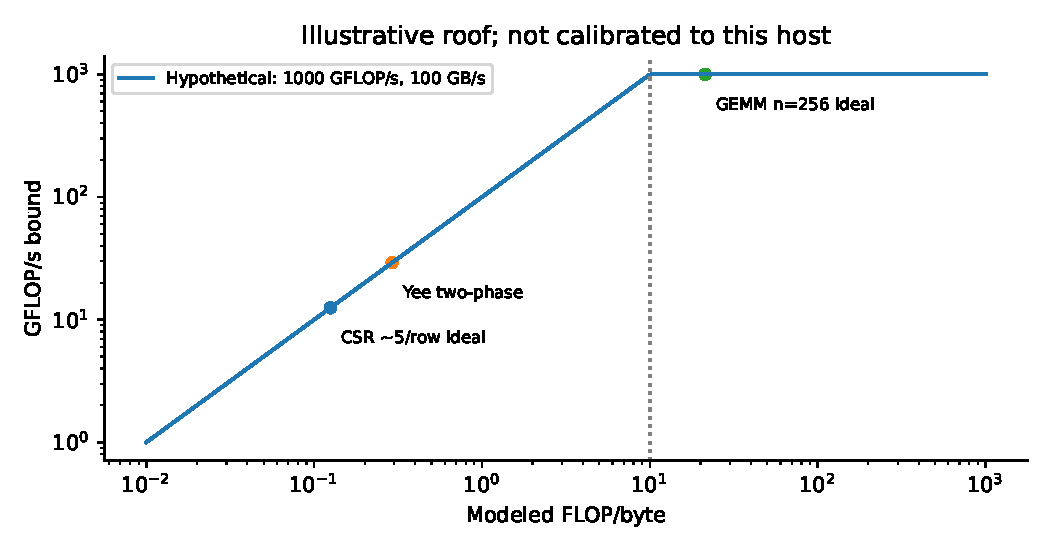
\includegraphics[width=.84\textwidth]{Vol0_Linear_Algebra_HPC/figures/roofline_model.pdf}}{}
\caption{Roofline for hypothetical hardware; neither the roof nor the byte model is a DRAM-counter measurement.}
\end{figure}
Calibration separately measures sustained bandwidth, precision-specific throughput, and actual traffic. Different cache levels can have different roofs. DRAM models do not describe cache-resident small arrays.
\costnote{Bandwidth-bound kernels benefit from reduced traffic, reuse, and layout improvements; compute-bound kernels benefit from vectorization and instruction efficiency. GFLOP/s diagnoses resource use, while total time at fixed error measures computational benefit.}
\coderef{roofline/kernels.py}
\aiexercise{For CSR with 32- and 64-bit indices, derive ideal-reuse and per-nonzero $x$-read traffic models. Compute intensities and identify omitted write-allocation effects.}{Given GEMM/SpMV times and array sizes, determine whether they can share one DRAM Roofline and identify missing measurements.}
\studyroute{Hardware-counter calibration and empirical hierarchical-Roofline tooling are omitted. See \cite{roofline,cuda}.}{arithmetic intensity; operational intensity; ridge point; sustained bandwidth; hierarchical Roofline}

\chapter{Computational and Memory Fingerprints of Discretizations}\label{v0ch:23}
\begin{chaptersummary}
Roofline analysis begins with an operator's work and data traffic. Comparing finite differences, finite volumes, FEM, DG, FR, and LBM shows how degrees of freedom, locality, order, and geometry shape reuse. These computational and access patterns form performance signatures, made concrete by the following Yee update and integrated experiments.
\end{chaptersummary}
\learninggoals{Construct work and access models; distinguish assembled and matrix-free operators; compare volume, face, streaming, and collision terms.}
\paragraph{Core Question}How does spatial discretization determine what a machine reads and computes?

\section{Finite Differences and Finite Volumes}
A three-dimensional seven-point Laplacian can be evaluated as
\[
 (\bm L u)_{ijk}
 =h^{-2}(u_{i+1,j,k}+u_{i-1,j,k}+u_{i,j+1,k}
 +u_{i,j-1,k}+u_{i,j,k+1}+u_{i,j,k-1}-6u_{ijk})
\]
Counting five neighbor additions, multiplication by 6, subtraction, and scaling gives 8 FLOPs. Seven reads and one write give 64 semantic bytes per double-precision output. Ideal spatial reuse approaches one read and one write, or 16 bytes, excluding write allocation. Spatial and temporal blocking improve within-step and cross-step reuse, subject to boundaries and dependencies.
Finite volumes combine gradient reconstruction, limiters, face Riemann fluxes, and residual accumulation. Unstructured faces introduce gathers/scatters. Computing each face once avoids duplicate fluxes but may require coloring, atomics, or buffers; independent cell traversal avoids write conflicts but repeats flux work. Compare at equal accuracy and conservation requirements.
\section{Finite Elements, DG, and FR}
Low-order assembled FEM may be dominated by sparse multiplication, while assembly also involves quadrature, geometry, and sparse accumulation. Matrix-free evaluation recomputes element actions, trading arithmetic for entry and index traffic.
For three-dimensional tensor elements with $n=p+1$ points per direction, a dense volume operator can cost $O(n^6)$; sum factorization reduces directional derivatives to $O(n^4)$:
\[
 (\partial_\xi u)_{ijk}=\sum_{\ell=0}^{p}D_{i\ell}u_{\ell jk}.
\]
Each direction uses $n^3$ length-$n$ dot products, totaling $3n^3(2n-1)$ FLOPs. Reading the input once and writing three derivatives gives approximately $32n^3$ bytes of field traffic, plus derivative matrices, geometry, and materials. Batching, register pressure, and faces change actual reuse.
DG volume terms, face fluxes, and liftings admit separate models; FR combines nodal derivatives with interface-flux corrections. Both exploit local matrix products on tensor grids. Correction functions, quadrature, and nodes determine their operator relationship, while energy or spectral estimates establish stability.
\conceptbridge{How can higher order be faster despite more operations per element?}{Higher order may improve reuse and reach a target error with fewer elements. It also changes unknown counts, face costs, and explicit stability limits. Evaluate spatial error, temporal error, and total step count together.}{High-order local work $\longrightarrow$ reuse and error changes $\longrightarrow$ total-cost comparison.}
\section{LBM Streaming and Collision}
Each lattice site stores $Q$ populations; BGK collision is
\[
 f_q^*=f_q-\tau^{-1}(f_q-f_q^{\rm eq}),\qquad
 f_q(\bm x+\bm c_q\Delta t,t+\Delta t)=f_q^*(\bm x,t).
\]
D2Q9, D3Q19, and D3Q27 have 9, 19, and 27 populations. Two-buffer streaming requires at least $2Q$ scalar reads/writes; double-precision D2Q9 gives 144 bytes/site before collision temporaries and boundaries.
SoA groups one population across sites; AoS groups populations at each site. Suitability depends on SIMD/SIMT mapping and collision implementation. Push writes postcollision values to neighbors; pull reads from neighbors. Injective periodic streaming avoids write conflicts, while complex boundaries require separate treatment.
\section{A Common Comparison}
\begin{center}\small
\begin{tabularx}{\textwidth}{lXX}
\toprule Method&Reuse and access&Typical limitations\\\midrule
FDM&Regular neighbors and cross-point reuse&Bandwidth, boundaries, time steps\\
FVM&Face geometry, reconstruction, fluxes&Irregular access, branches, accumulation\\
FEM&Local quadrature or sparse products&Different assembly/application paths\\
DG&Tensor volume and face data&Registers, lifting, stable step size\\
FR&Point derivatives and flux corrections&Nodes, correction functions, face exchange\\
LBM&Population streaming and collision&Layout, storage, complex boundaries\\
FDTD&Staggered curl stencils&Two-phase dependencies, bandwidth, dispersion\\\bottomrule
\end{tabularx}
\end{center}
\costnote{The table uses access patterns to locate bottlenecks. Method comparisons fix the physical problem, error, precision, hardware, and parallel scale. For NumPy implementations, include temporary-array traffic in addition to the ideal fused-kernel model.}
\coderef{roofline/kernels.py; dg_fr/transport.py; lbm/stream_collision.py}
\aiexercise{List operations and reads/writes for seven-point Laplacian, tensor derivatives, and D2Q9 streaming. Identify cache-reusable reads.}{Compare first-order upwind FVM and high-order DG for the same periodic sine transport, recording spatial error, steps, and total time. Keep LBM fluid physics distinct from arbitrary scalar transport.}
\studyroute{General curved-element sum factorization and FR energy-stability proofs are omitted. See \cite{hesthaven,vcjh,frdisp,roofline}.}{sum factorization; matrix-free FEM; DG volume surface; FR correction; LBM SoA AoS}

\chapter{Yee-FDTD: Discrete Structure and Performance}\label{v0ch:24}
\begin{chaptersummary}
Volume II established compatible discretizations of Maxwell evolution and constraints. Yee degrees of freedom, staggered time levels, and curl structure now turn topological identities into array updates and explicit work and traffic models. The discrete complex, phase relations, and two-phase dependencies define the constraints within which performance is optimized.
\end{chaptersummary}
\learninggoals{Write Yee updates and constraints; distinguish incidence from material Hodge operators; calculate three traffic models and check dispersion and energy.}
\paragraph{Core Question}How can Yee bottlenecks be identified while preserving Maxwell structure?

\section{Degrees of Freedom, Materials, and the Grid}
For stationary, nondispersive isotropic media,
\[
 \varepsilon\partial_t\bm E=\nabla\times\bm H-\bm j,\qquad
 \partial_t\bm B=-\nabla\times\bm E,\qquad \bm B=\mu\bm H.
\]
The coefficients $\varepsilon,\mu$ remain explicit in material and wave-speed relations. On a cubic grid, $E_x$ lies at $(i+\tfrac12,j,k)$, with $E_y,E_z$ obtained cyclically; $B_x$ lies at $(i,j+\tfrac12,k+\tfrac12)$, with the others cyclic. $E$ uses integer times and $B$ half-integer times.

\begin{figure}[H]\centering
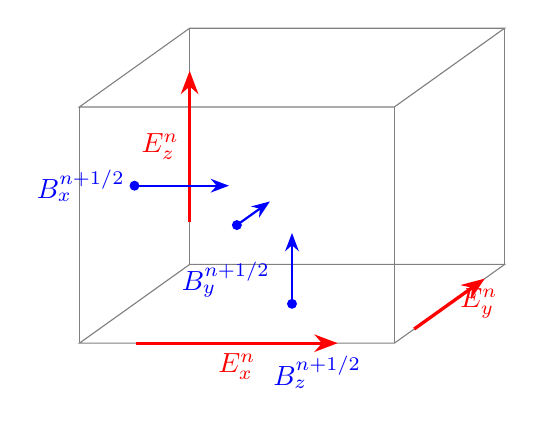
\begin{tikzpicture}[x={(4cm,0cm)},y={(1.4cm,1cm)},z={(0cm,3cm)},>=Stealth]
\foreach \z in {0,1}{\draw[gray] (0,0,\z)--(1,0,\z)--(1,1,\z)--(0,1,\z)--cycle;}
\foreach \x in {0,1}{\foreach \y in {0,1}{\draw[gray] (\x,\y,0)--(\x,\y,1);}}
\draw[very thick,red,->](.18,0,0)--(.82,0,0) node[midway,below]{$E_x^n$};
\draw[very thick,red,->](1,.18,0)--(1,.82,0) node[midway,right]{$E_y^n$};
\draw[very thick,red,->](0,1,.18)--(0,1,.82) node[midway,left]{$E_z^n$};
\fill[blue] (0,.5,.5) circle(1.8pt);
\draw[blue,thick,->](0,.5,.5)--(.3,.5,.5);
\node[blue,anchor=east] at (0,.5,.5) {$B_x^{n+1/2}$};
\fill[blue] (.5,0,.5) circle(1.8pt);
\draw[blue,thick,->](.5,0,.5)--(.5,.3,.5);
\node[blue,anchor=north] at (.5,-.1,.42) {$B_y^{n+1/2}$};
\fill[blue] (.5,.5,0) circle(1.8pt);
\draw[blue,thick,->](.5,.5,0)--(.5,.5,.3);
\node[blue,anchor=north] at (.58,.5,-.18) {$B_z^{n+1/2}$};
\end{tikzpicture}
\caption{Representative edge electric and face magnetic components in a cubic cell. Arrows indicate component directions; not all edge/face unknowns are shown.}
\end{figure}

Point components are samples on a uniform grid. Integral unknowns are edge circulations $e_\ell=\int_\ell E$ and face fluxes $b_f=\int_f B$. Lengths, areas, and materials connect the representations; point arrays are not dimensionless incidence matrices.
\section{Topology and Matrix-Free Updates}
Incidence matrices $G,C,D$ satisfy $CG=0,DC=0$. With compatible primal/dual grids and boundary pairing,
\[
 \dot{\bm b}=-C\bm e,\qquad
 M_\varepsilon\dot{\bm e}=C^TM_{\mu^{-1}}\bm b-\bm j_h .
\]
$C$ encodes orientation; $M_\varepsilon,M_{\mu^{-1}}$ encode metric and material data. Uniform orthogonal Yee grids admit diagonal material actions. Thus $\partial_t(D\bm b)=0$. With dual-divergence convention $D_e=-G^T$, charge is $\bm q=D_eM_\varepsilon\bm e$ and continuity requires $\dot{\bm q}=-D_e\bm j_h$, with compatible boundary fluxes.
Define forward differences $\delta_\alpha^+$ and backward differences $\delta_\alpha^-$. On a periodic uniform grid,
\[
 B_x^{n+1/2}=B_x^{n-1/2}
 -\Delta t(\delta_y^+E_z^n-\delta_z^+E_y^n),
\]
\[
 E_x^{n+1}=E_x^n+\frac{\Delta t}{\varepsilon}
 [\delta_y^-H_z^{n+1/2}-\delta_z^-H_y^{n+1/2}-j_x^{n+1/2}],
\]
with cyclic counterparts. This is a block-sparse action without CSR assembly. Explicit matrices remain useful for small spectral checks, implicit integration, and operator comparisons. The execution order is
\begin{quote}\ttfamily\small
for each time step:\\
\quad exchange required E halos\\
\quad B\_half = B\_half - dt * curl\_forward(E)\\
\quad exchange required B\_half halos\\
\quad E = E + dt * curl\_backward(B\_half)
\end{quote}
\conceptbridge{Why can curl updates not be changed arbitrarily to in-place operations?}{Both curls must retain consistent time levels and spatial orientation. The magnetic half-step reads old electric fields; the electric step reads new magnetic fields. Overwriting unread values changes the operator, stability, dispersion, and constraints.}{Staggered unknowns $\longrightarrow$ two-phase dependency graph $\longrightarrow$ admissible fusion and synchronization.}
\section{Auditable Work and Traffic}
For source-free, constant-coefficient vacuum with precomputed inverse spacings, each component uses two differences, two scalings, a subtraction, a $\Delta t$ multiplication, and an update: 7 FLOPs, or 42 per six-component cell-step. An FMA counts as two FLOPs.
This counts separately formed directional differences. On an isotropic equal-spacing grid, precombining $\Delta t/h$ gives three subtractions, one scaling, and one update per component: 5 FLOPs, or 30 per cell-step. The CUDA/MPI code uses this form. Count the implemented work; do not assign 42 FLOPs to the fused kernel.
For double precision, excluding materials and sources:
\[
\begin{array}{l|r|r}
\text{Model}&\text{bytes/cell-step}&I\ (\text{FLOP/byte})\\\hline
\text{Four neighbors+self read+write}&288&42/288\\
\text{Ideal reuse within each phase}&144&42/144\\
\text{Six fields resident for full step}&96&42/96
\end{array}
\]
The three values describe traffic under specified reuse assumptions. Actual DRAM traffic also depends on caches, write allocation, temporaries, boundaries, and coefficient access. For large two-phase arrays, working-set size determines whether whole-step residency is feasible.
Six SoA arrays support contiguous spatial access by neighboring threads. GPU execution can use separate $B/E$ launches, further split by component if needed. Registers, launch cost, and global synchronization determine the tradeoff. Shared memory helps only when it reduces actual repeated movement without unduly reducing parallelism.
\section{Stability, Dispersion, and Acceptance}
With vacuum wave speed $c=(\varepsilon\mu)^{-1/2}$, the uniform three-dimensional condition is
\[
 c^2\Delta t^2(h_x^{-2}+h_y^{-2}+h_z^{-2})\le1.
\]
Periodic Fourier modes satisfy
\[
 \frac{\sin^2(\omega_h\Delta t/2)}{c^2\Delta t^2}
 =\sum_\alpha\frac{\sin^2(k_\alpha h_\alpha/2)}{h_\alpha^2}.
\]
CFL controls numerical growth, while the dispersion relation describes phase propagation. Evaluate fixed-distance propagation errors together with direction, resolution, and total step count.
For normalized periodic vacuum, an exact-arithmetic invariant is
\[
 {\cal H}^n=\frac12\norm{E^n}^2+
 \frac12\langle B^{n-1/2},B^{n+1/2}\rangle
\]
with the appropriate volume weights. This is a modified staggered energy, not a sum of squares at unrelated times. Its relation to physical energy under stable time steps must be specified.
\costnote{Record initial phase, final physical time, error, $\diverg_h B$, charge residual, modified energy, and advance time. Include nontrivial random-field curl--divergence checks, not just a transverse wave. Periodic lossless modes have unit-modulus amplification in the stable range; boundaries, material losses, and filtering may add dissipation and require separate records.}
\coderef{fdtd/yee.py}
\aiexercise{Derive neighboring indices for $B_x$ and $E_x$ from their locations. Verify $D C=0$ term by term and identify the length/area factors.}{Derive Yee dispersion and CFL from Fourier updates. Compare modified staggered energy with sums of squares at different times.}
\crossref{Volume II explains geometry and constraints; the material matrices, traffic, and time levels here support Chapters 25, 28, and 29.}
\studyroute{PML, dispersive materials, curvilinear Hodge operators, and PEC details are omitted. See \cite{yee,cuda}.}{Yee staggered grid; incidence matrix; discrete Hodge; numerical dispersion; modified energy}

\chapter{Time Integration and Total Solution Cost}\label{v0ch:25}
\begin{chaptersummary}
Spatial throughput gives the cost of one call; time integration determines call counts and implicit-solve work. A common framework connects RK, staggered integration, ADER, CERK, LTS, and IMEX to stability, phase accuracy, and structure preservation. At a specified error and final time, step size, stages, solves, and communication jointly determine total cost.
\end{chaptersummary}
\learninggoals{Relate semidiscrete spectra to stability regions; distinguish symplecticity from energy conservation; analyze high-order, local-step, and stiff-splitting costs.}
\paragraph{Core Question}Why can a simulation remain slow when one spatial evaluation is fast?

\section{Method of Lines and Stability Regions}
Spatial discretization gives $M\dot{\bm u}=\bm R(\bm u)$. Each explicit RK stage applies $M^{-1}\bm R$, cheaply for local or diagonal mass matrices. For $\dot y=\lambda y$, one step is $y^{n+1}=R(z)y^n$ with $z=\Delta t\lambda$; absolute stability requires $|R(z)|\le1$. Classical RK4 has
$R(z)=1+z+z^2/2+z^3/6+z^4/24$. Spectra, nonnormality, and energy estimates jointly constrain usable steps.
For purely imaginary $\lambda$, forward Euler has $|1+\mathrm i\omega\Delta t|>1$, producing modal growth. The time integrator's stability region is therefore part of the complete energy analysis.
\section{Staggering, Symplecticity, and Phase}
Yee/leapfrog staggers suitable split systems and is conditionally stable. St\"ormer--Verlet is second-order symplectic for separable Hamiltonian systems. Implicit midpoint
\[
 \frac{\bm u^{n+1}-\bm u^n}{\Delta t}
 =A\frac{\bm u^{n+1}+\bm u^n}{2}
\]
exactly preserves a quadratic energy when $A^TQ+QA=0$ with fixed SPD $Q$. It is symplectic for general Hamiltonian systems, but symplecticity does not generally imply exact preservation of the original Hamiltonian.
For $\lambda=\mathrm i\omega$, midpoint has phase frequency
$\omega_h=2\arctan(\omega\Delta t/2)/\Delta t$. Stable amplitude can accompany accumulated phase error; inaccurate linear solves also affect preservation.
\section{ADER, CERK, and LTS}
ADER constructs high-order time representations using element-local space--time prediction, followed by interface space--time flux correction. Prediction can improve local reuse; cost, stability, and order depend on the implementation.
CERK denotes continuous explicit Runge--Kutta, adding an within-step approximation
\[
 \bm u(t_n+\theta\Delta t)
 \approx\bm u_n+\Delta t\sum_i b_i(\theta)\bm k_i,\quad0\le\theta\le1.
\]
Within-step accuracy follows the continuous-extension order conditions; endpoint accuracy follows those of the RK update. Coupling and output therefore check the two orders separately.
LTS groups elements by size or wave speed. Conservation requires one shared time-integrated interface flux, with consistent fine-step accumulation and coarse correction. Interpolation, flux registers, scheduling, and imbalance add cost.
\section{IMEX and Stiff Sources}
Split $\dot{\bm u}=F(\bm u)+G(\bm u)$, treating propagation explicitly and stiff sources implicitly. Additive RK stages are
\[
 U_i=\bm u^n+\Delta t\sum_{j<i}\widetilde a_{ij}F(U_j)
                  +\Delta t\sum_{j\le i}a_{ij}G(U_j),
\]
The endpoint uses separate explicit and implicit weights. Order and stability depend on the paired tableaux and coupling conditions.
Conductive Maxwell may use $G_E=-\sigma E/\varepsilon$. A first-order split example is
\[
 E^{n+1}=\frac{E^n+\Delta t\,(\curl H)^n/\varepsilon}
 {1+\Delta t\,\sigma/\varepsilon}.
\]
This illustrates cheap local implicit damping. If propagation uses forward Euler, the $\sigma=0$ wave limit remains unsuitable. Choose an IMEX pair compatible with the hyperbolic explicit stability region. Global diffusion or coupled implicit sources may reintroduce large linear systems.
\conceptbridge{Why do high-order or implicit methods not automatically reduce cost?}{Higher order changes stage counts and error constants; implicit treatment changes stability limits but adds solves. Local steps change scheduling and communication. At equal error requirements, determine usable steps, total steps, and the complete per-step execution graph together.}{Stability and accuracy $\longrightarrow$ usable time step $\longrightarrow$ stages, solves, and communication.}
\section{Minimal Comparisons}
For periodic sine transport, compare RK4, second-order methods, and staggered wave updates. For $\dot y=\mathrm i\omega y-\sigma y$, compare explicit/IMEX stability and phase. Assess error at a fixed final time rather than only plotting $|R|$.
\costnote{$T_{\rm total}=T_{\rm setup}+N_tT_{\rm step}+T_{\rm output}$, where $T_{\rm step}$ includes all stages, implicit solves, and communication. ADER and LTS trade extra local work for opportunities to reduce global updates. CERK supplies time-aligned states; interface fluxes and the combined stability region control conservation and stability.}
\aiexercise{Derive midpoint's phase frequency from its amplification factor. Quantify phase error after one hundred periods and compare RK4.}{Write shared flux integrals and fine-step accumulation for adjacent unequal-step elements. Explain why interpolated boundary values alone do not ensure conservation.}
\studyroute{ADER predictors, CERK order conditions, and high-order IMEX tableaux are omitted. See Volume II's time-integration chapter and \cite{hesthaven,ader,cerk,imex}.}{method of lines; symplectic integrator; ADER; continuous explicit Runge Kutta; conservative LTS; IMEX additive RK}

\chapter{Memory Hierarchies and Operator Implementation}\label{v0ch:26}
\begin{chaptersummary}
Ideal traffic estimates set reuse targets; implementation determines the storage levels through which data actually move. Registers, caches, and DRAM connect to layout, blocking, fusion, and SIMD through temporaries, dependencies, and access paths. Optimization reduces movement at the limiting level and is evaluated under common accuracy and timing conventions.
\end{chaptersummary}
\learninggoals{Analyze strides and cache reuse; explain fusion, blocking, SIMD, and matrix-free tradeoffs; design fair timings.}
\paragraph{Core Question}Why does a program repeatedly move data that ideally need only one read?

\section{Hierarchy, Locality, and Layout}
Registers are close to execution units; L1/L2/L3 caches provide increasing capacity, and DRAM supplies main capacity. Sharing arrangements depend on architecture. Contiguous access improves cache-line use and prefetching; large strides and random gathers may waste transactions. Working-set size determines which reuse survives.
In C-order three-dimensional arrays, the final index is contiguous. Align inner loops and thread mappings accordingly. SoA often favors cross-point vectorization; AoS may favor using every component at a point; AoSoA combines these within blocks. Judge layouts by the actual kernel.
\section{Fusion and Blocking}
Evaluating $w=a u+b v$ through two temporary arrays adds writes and reads. Fusion can read $u,v$ and write $w$ directly, but increases live registers; excessive fusion can cause spills.
Spatial blocking retains neighboring stencil planes. Temporal blocking reuses subdomains across steps while respecting dependence cones and expanded halos. Two-phase Yee or multistage RK cannot be fused arbitrarily across steps without synchronization.
Tensor DG can reuse derivative matrices and batch elements. Keeping three derivatives and fluxes simultaneously may exceed register/cache capacity. Matrix-free evaluation reduces sparse indexing but repeats geometry work; mixed precision additionally requires error analysis.
\conceptbridge{Why can zero-copy or matrix-free code remain slow?}{Avoiding explicit copies or matrix entries removes only one class of work. Cache misses, hidden temporaries, migration, and extra arithmetic may still dominate. Infer traffic from actual access paths, not interface names.}{Storage representation $\longrightarrow$ actual access paths $\longrightarrow$ per-level resource use.}
\section{SIMD and Minimal Experiments}
SIMD applies one instruction to several elements, requiring independent iterations, suitable layout/alignment, and manageable branching. Vectorization reports, assembly, and counters are more reliable than source appearance.
Compare contiguous and strided seven-point traversal, D2Q9 SoA/AoS, and explicit-Kronecker versus sequential tensor contractions. Warm up, retain outputs, repeat timings, and report statistics. Separate large arrays from cache-resident cases.
\costnote{Report allocation and kernel times separately, comparing preallocated and dynamically allocated implementations within a common timing scope. Individual NumPy operations invoke compiled kernels; fusion across operations depends on the execution strategy.}
\coderef{roofline/kernels.py; lbm/stream_collision.py; dg_fr/transport.py}
\aiexercise{List every NumPy seven-point temporary and its lifetime. Compare resulting bytes with Chapter 23's fused lower bound.}{Design working sets fitting L1, fitting L3, and exceeding last-level cache. Explain why one undifferentiated bandwidth cannot describe them all.}
\studyroute{Cache replacement, compiler vectorization, and microarchitectural port analysis are omitted. See \cite{roofline,cuda}.}{cache blocking; loop fusion; temporal blocking; SIMD; AoSoA; working set}

\chapter{Parallel Throughput on CPUs and GPUs}\label{v0ch:27}
\begin{chaptersummary}
Layout controls a single execution stream; parallel performance also requires sufficient independent work and resources. This chapter connects CPU threads and GPU SIMT to occupancy, coalescing, and device residency. Evaluate throughput, dependencies, launch, and migration together, using end-to-end timing to assess acceleration.
\end{chaptersummary}
\learninggoals{Explain NUMA and false sharing; distinguish SIMD/SIMT; assess coalescing, occupancy, and transfer amortization.}
\paragraph{Core Question}Why do more threads or higher occupancy not necessarily shorten runtime?

\section{CPU Threads and Memory Placement}
Multicore execution distributes elements, rows, or grid blocks among threads. OpenMP loops need conflict-free writes or synchronization. Binding and first touch determine NUMA page placement; cross-socket access changes latency and bandwidth. Threads writing distinct variables on one cache line can still cause false sharing. Blocking and padding separate hotspots. SIMD and multicore threading are complementary levels.
On hybrid-core processors, thread performance, affinity, and power state affect short experiments. The records therefore include CPU model, available logical processors, and BLAS configuration; sustained all-core throughput requires calibration with a corresponding workload.
\section{GPU Execution Resources}
CUDA groups threads into blocks, schedules blocks onto SMs, and executes warps in SIMT fashion.\cite{cuda}
Contiguous threads accessing contiguous elements favor coalescing. Divergence, irregular gathers, and insufficient parallelism reduce utilization. Registers and shared memory limit resident blocks/warps. Occupancy measures residency, not performance; raising it while sacrificing reuse or causing spills may be counterproductive.
SpMV short and long rows have different workloads. DG elements can be batched into small matrix kernels. Yee/LBM should first align spatial indexing, then consider shared caching. Fixed launch overhead can dominate small problems.
\section{Transfers, Asynchrony, and Residency}
\[
 T_{\rm accelerator}=T_{\rm H2D}+T_{\rm kernels}
 +T_{\rm D2H}+T_{\rm synchronization}.
\]
Keep evolving fields, geometry, and preconditioner data on the device when possible. Copy/compute overlap requires hardware support, appropriate streams, and buffer management. An asynchronous call's return is not completion. Use device events or synchronization, separating first launch, steady kernels, and transfer-inclusive totals.
Unified memory supplies shared addressing and demand migration, not the elimination of data movement. Faults, granularity, and residency still matter. Compare explicit prefetch and ownership policies with explicit-transfer measurements.
\conceptbridge{Why can timing an asynchronous call with a CPU clock produce a fictitious speedup?}{The host often only enqueues work. Stop timing after the corresponding device work completes, and state whether transfer and initialization are included.}{Host submission $\longrightarrow$ device execution $\longrightarrow$ completion synchronization and valid timing.}
\section{A Reproducible Interface}
The CUDA program compares single-component AoS/SoA access, advances periodic Yee fields in two phases, and checks results on the host. Compilation, device availability, and numerical validation are recorded separately; timings are produced after device execution. A complete experiment also records model, driver, precision, block configuration, registers, device bandwidth, and transfer scope.
\costnote{GPU benefits depend on size and residency. Sparse triangular dependencies, reductions, and small kernels may limit acceleration. CPU implementations should also avoid oversubscription between BLAS and outer threads.}
\coderef{gpu/yee_layout.cu}
\aiexercise{List warp addresses for SoA and AoS $E_x$ updates. Estimate transaction use and identify quantities requiring profiler confirmation.}{Design timings including transfers, warmup, repetitions, and synchronization. Derive how many steps amortize one device migration.}
\studyroute{Device-specific pipelines and autotuning are omitted. See \cite{cuda}.}{OpenMP; NUMA first touch; false sharing; SIMT; coalescing; occupancy; device residency}

\chapter{Distributed Computing and Communication Cost}\label{v0ch:28}
\begin{chaptersummary}
As single-node computation accelerates, halo exchange, global dot products, and coarse-level communication enter the critical path. Message latency and volume complement compute and memory Roofline analysis, explaining scaling, progress, and overlap. Operator dependencies identify communication that can be hidden; timing establishes whether that overlap is realized.
\end{chaptersummary}
\learninggoals{Build an alpha--beta model; distinguish halos and allreduce; explain overlap, pipelining, and coarse-level bottlenecks.}
\paragraph{Core Question}Why does speedup saturate even when local computation is fast?

\section{Communication and Scaling}
A communication phase may be approximated by
\[
 T_{\rm comm}\approx n_{\rm msg}\alpha+V/B_{\rm net},
\]
where $\alpha$ is effective message-start latency, $V$ the explicitly defined volume, and $B_{\rm net}$ effective bandwidth. Protocol, topology, congestion, and concurrency affect parameters. Nonoverlapped costs add; ideal overlap suggests a more optimistic lower bound:
\[
 T\gtrsim\max(F/P_{\rm peak},Q/B_{\rm mem},T_{\rm comm}).
\]
This estimate describes a resource lower bound under ideal overlap; communication progress, contention, and dependency chains determine the realized time.
Strong scaling fixes global size. As local cubic side $\ell$ decreases, volume work is $O(\ell^3)$ and face exchange $O(\ell^2)$, increasing surface-to-volume ratio. Weak scaling fixes local work but still encounters global reductions, network effects, and coarse levels.
\section{Halos, Reductions, and Overlap}
Regular stencils exchange neighboring faces; FVM/DG exchange face values or traces, with higher order increasing face data and local work. Yee exchanges follow magnetic/electric phase dependencies. Krylov adds dot-product allreduces to operator halos. Short CG recurrences retain global synchronization; GMRES orthogonalization can add reductions.
Post nonblocking receives/sends, compute halo-independent interiors, wait, then update boundaries. Actual progress and overlap depend on MPI and runtime configuration and require measurement.\cite{mpi}
Pipelined Krylov overlaps reductions with computation. Communication-avoiding block or s-step schemes reduce synchronization but may increase basis ill-conditioning, work, and residual drift. Numerical stability requires simultaneous checks.
\conceptbridge{Why can equal communication volumes have different costs?}{Many small messages are latency-sensitive; fewer large messages are more bandwidth-sensitive. Critical-path placement, progress, and contention also differ. Bytes alone do not describe these dependencies.}{Message counts and sizes $\longrightarrow$ progress and dependencies $\longrightarrow$ critical-path time.}
\section{A Minimal MPI Experiment}
The program partitions a three-dimensional periodic field in one direction, exchanges faces using \texttt{Sendrecv} or \texttt{Irecv/Isend+Waitall}, and checks the seven-point operator on a global Fourier mode. Records include ranks, local size, maximum-rank time, and error. Single-host runs verify MPI semantics; cross-node runs measure network scaling. Multidimensional partitioning additionally requires six-face exchange and a partition strategy.
\costnote{AMG coarse levels have shrinking local work and increasing communication ratios, sometimes requiring process aggregation. Time operators, preconditioners, reductions, and I/O separately. Strong-scaling comparisons use the slowest rank.}
\coderef{mpi/halo.cpp}
\aiexercise{For an $n^3$ grid split into $p$ approximately cubic subdomains, derive local work, six-face halo bytes, and surface-to-volume ratio.}{Draw a nonblocking halo event graph, marking overlappable interiors and dependent boundaries. Design a test of actual progress.}
\studyroute{Network-topology models, pipelined-Krylov error analysis, and cross-node tuning are omitted. See \cite{mpi,petsc}.}{alpha beta model; strong scaling; weak scaling; halo exchange; allreduce; pipelined Krylov; MPI progress}

\chapter{Integrated Cases Across the Volumes}\label{v0ch:29}
\begin{chaptersummary}
The preceding chapters separated discrete operators, algebraic algorithms, and execution costs. Reproducible experiments now reconnect them: first verify the model, errors, and constraints, then record solution and data-movement costs. Comparing total time for a common problem and target error turns kernel analysis into an integrated computational decision.
\end{chaptersummary}
\learninggoals{Create consistent experiment records; complete Maxwell and high-order transport cases; distinguish kernel benchmarks, complete solves, and cross-model comparisons.}
\paragraph{Core Question}How can we establish that a faster implementation still solves the same problem?

\section{Krylov and AMG: From Poisson to Preconditioning}
Start with Volume I's two-dimensional Dirichlet Poisson discretization. Manufacture algebraic data to check direct, CG, and preconditioned true residuals; then use a continuous exact solution to assess discretization error. Record unknowns, $\nnz$, ordering, fill, setup, iterations, time, and error.
Use the algebraically manufactured right-hand side $\bm b=A\bm x_*$ to check the linear solver, then a continuous analytic solution to test PDE convergence. The code records these error levels separately. Multiple right-hand sides reuse the same factors to expose setup amortization, while the two-level AMG example verifies coarse-space correction.
Separate Krylov SpMV, preconditioning, dot products, and orthogonalization. Record AMG smoothing, restriction, coarse solve, and interpolation by level. At small sizes, fewer iterations may not offset setup and Python overhead; at large sizes, coarse communication and reductions can change the comparison. Serial teaching hierarchies do not measure distributed AMG scaling.
\section{Complete Maxwell Evolution}
On the periodic unit cube with vacuum $c=1$, use the right-going transverse wave
\[
 E_y(x,t)=\sin(2\pi(x-t)),\qquad B_z(x,t)=\sin(2\pi(x-t)).
\]
All other components vanish. Initialize the magnetic field at its own spatial locations and $t=-\Delta t/2$, choosing
$\Delta t\le\nu h$, $\nu<1/\sqrt3$, and adjusting the step to reach the same $T$ exactly. Compare $L^2$ error, phase, steps, and time on two grids. Half-time initial data must not be treated as full-time values.
The CPU code also computes curls of random edge fields, checking divergence and monitoring $\diverg_h B$ and modified energy. The source-free electric-divergence test represents zero charge; sources require compatible current and continuity updates.
\begin{figure}[htbp]\centering
\IfFileExists{Vol0_Linear_Algebra_HPC/figures/convergence.pdf}{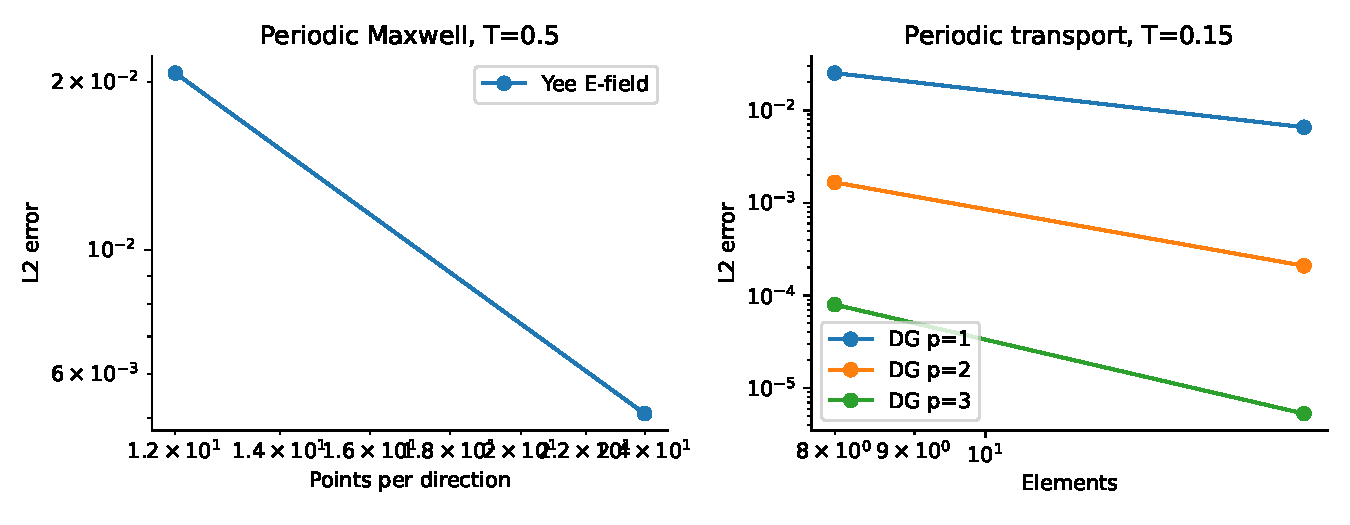
\includegraphics[width=.88\textwidth]{Vol0_Linear_Algebra_HPC/figures/convergence.pdf}}{}
\caption{Measured CPU convergence data for Yee transverse waves and periodic transport. Error definitions and parameters accompany the records.}
\end{figure}
GPU execution preserves SoA, phase order, and initial data. MPI exchanges required fields per phase before interior/boundary work. The CUDA full-field program provides a device path; the MPI solver includes phase halos and global constraints. The appendix and data record execution scope; cross-node and multi-GPU coupling can then be measured under the same error and constraint conventions.
\section{Complete High-Order DG and the FR Interface}
For $u_t+u_x=0$ with periodic $u(x,0)=\sin(2\pi x)$, use elementwise Legendre modes
$u_h=\sum_{m=0}^{p}\widehat u_mP_m(\xi)$. The weak form is
\[
 \frac h2 M\dot{\widehat{\bm u}}
 =S\widehat{\bm u}-\bm\phi(1)\widehat f_R
                         +\bm\phi(-1)\widehat f_L,\quad
 M_{mm}=\frac2{2m+1},\quad S_{m\ell}=\int_{-1}^{1}P'_mP_\ell.
\]
For positive speed, upwinding takes the left trace. Volume terms, face fluxes, and diagonal mass inversion are directly implementable. RK4 with conservative steps compares $p=1,2,3$ and element counts in error, unknowns, steps, and time.
At the two $p=1$ Lobatto endpoints, the FR test uses
$g_L=(P_2-P_1)/2$, $g_R=(P_2+P_1)/2$
Construct derivative corrections and verify equivalence with nodal DG under the same exact-mass and quadrature conventions. For other correction functions, compare their lifting and volume operators directly. Three-dimensional tensor derivatives are also checked against dense Kronecker application to verify sum factorization.
MPI partitions elements, exchanges upwind traces at every RK stage, and retains local mass inversion. GPU optimization can batch same-order elements, reuse derivative matrices, and separate volume/face work. Increasing order raises register demand and volume-to-face ratio. Executed GPU checks currently cover Yee and layout; a complete DG GPU port is a separate extension.
\conceptbridge{Why can higher kernel throughput accompany a slower complete DG run?}{High-order local work increases intensity but also changes stable steps, stages, and error. Local throughput becomes an end-to-end benefit only through the element and step counts required for target accuracy.}{Kernel reuse $\longrightarrow$ accuracy and stable step $\longrightarrow$ cost to physical final time.}
\section{Access Comparisons: FDM, FVM, FEM, and LBM}
First-order upwind FVM solves the same periodic transport problem as DG, enabling error and total-time comparisons. Seven-point FDM, Yee, DG tensors, LBM streaming and collision, and CSR/GEMM expose different access patterns. Cross-model update rates describe implementation signatures; method selection uses a common physical problem and target error.
FEM checks assembled against local matrix-free actions. FVM/DG checks shared-flux conservation; LBM checks periodic mass. Accept correctness before timing.
\subsection{Regular and Staggered Stencils}
Seven-point FDM outputs one scalar field per application; Yee updates six staggered components in two phases. Both support contiguous indexing and halos, but equal site counts imply neither equal unknowns nor equal physics. Distinguish the 8-FLOP Laplacian, 42-FLOP difference-based Yee, and 30-FLOP fused Yee, stating traffic assumptions.
\subsection{Adjacency, Irregular Access, and Geometry}
The FVM case renumbers nonuniform periodic cells, gathers states through left/right face indices, computes fluxes, and accumulates residuals. Verify permutation equivalence and zero volume-weighted residual sum. This isolates numbering and gather/scatter. General unstructured meshes additionally require normals, areas, reconstruction neighborhoods, and graph partitioning. MPI exchanges follow partition-crossing faces, not a presumed fixed array-neighbor pattern.
\subsection{Local Matrices and Population Layout}
One-dimensional P1 FEM compares CSR with elementwise difference accumulation under identical boundary elimination. LBM separately times streaming, collision, and complete steps. Streaming tests check push/pull and AoS/SoA equality; periodic BGK checks mass. Collision live variables and boundary branches also influence GPU occupancy, which a CPU layout test alone cannot predict.
\paragraph{The Eight Case Interfaces}
FDM--Yee stencils, FVM adjacency, DG/FR volume/face structure, LBM streaming/collision, Krylov, AMG, complete Maxwell, and complete high-order DG cover eight performance interfaces. Code and appendices specify acceptance criteria and execution scopes.
\section{Common Acceptance and Selection}
\begin{center}\small
\begin{tabularx}{\textwidth}{lX}
\toprule Dimension&Required record\\\midrule
Physics/discretization&Equations, boundaries, initial data, $T$, mesh, order, unknowns\\
Accuracy&Space/time error, phase, true residual, conservation, constraints\\
Algorithmic work&Steps, stages, iterations, preconditioning, hierarchy complexity\\
Resources&Array/factor storage, modeled FLOPs/traffic, messages, reductions\\
Timing scope&Inclusion of setup, advance, transfer, communication, checks, output\\\bottomrule
\end{tabularx}
\end{center}
\costnote{Fixed-unknown comparisons analyze implementations; fixed-error comparisons select methods. Report both. Small CPU tests validate the workflow; large-scale optimization requires representative working sets, parallel scale, and counters.}
\coderef{run_all.py; run_accelerators.py; fdtd/yee.py; dg_fr/transport.py}
\aiexercise{Run the experiments and plot error against time and unknown count from JSON. Check that physics, final time, and error norm agree within each comparison.}{Choose an error threshold and search mesh, order, and time step jointly for Yee or DG, including setup, communication, and output in the budget.}
\studyroute{Cross-node benchmarks and engineering-scale complex boundaries are further experiments. The experiment guide supplies reproduction commands and timing conventions. References: \cite{yee,hesthaven,roofline}.}{verification versus validation; manufactured solution; error versus cost; constraint preservation; time to solution}

\appendix
\chapter{Reproduction and Measurement Conventions}
From the repository root, run \texttt{make vol0-examples} to generate CPU experiments, figures, and JSON; use \texttt{make vol0-en} to build this edition. Dependencies are Python, NumPy, SciPy, Matplotlib, and XeLaTeX. BLAS defaults to one thread, keeping thread configuration separate from algorithm comparisons.
\par
Shared \path{results/measurements.json} records environment, parameters, timing, residuals, and errors; \path{results/validation.json} records numerical assertions. Byte counts use explicit work models. A null \texttt{dram\_bytes\_measured} means no hardware counters were used; effective bandwidth inferred from modeled bytes is not measured DRAM bandwidth.
\par
GPU and MPI sources are under \path{gpu/} and \path{mpi/} in the shared code directory. Experiments record compilation, numerical device validation, and cross-node performance as separate evidence levels. Commands and timing conventions appear in \path{docs/experiments.md}. Figures come from the code; timings refer to the recorded implementation, workload, and hardware configuration.
\section{A Common Error and Cost Record}
Record equations, boundaries, initial data, physical final time, mesh/order, unknowns, step size/count, precision, error norms, constraints, setup, advance time, hardware, and threads. Fixed-grid throughput and fixed-error total time answer different questions.
\section{Transferability}
Recalibrate after changes to processor, power mode, threads, compiler, or libraries. Cache-resident arrays use roofs for the corresponding cache level; implementations with NumPy temporaries include intermediate reads and writes in their traffic model. Distributed experiments additionally record network, binding, message size, and reduction strategy.
\section{Recorded Numerical Results}
These tables are generated from the shared JSON records, not from new runs. CPU: Intel Core Ultra 7 155H; NumPy 1.26.4; SciPy 1.15.3. Double precision and single-thread BLAS. Times describe these implementations and small workloads.
\begin{center}\small\begin{tabular}{lrrrrr}\toprule
Case & Cells/elements & $p$ & Steps & $L^2$ error & Advance/s\\\midrule
Yee & 12 & -- & 14 & 2.076e-02 & 1.424e-03\\
Yee & 24 & -- & 27 & 5.094e-03 & 8.223e-03\\
DG & 8 & 1 & 44 & 2.523e-02 & 2.015e-03\\
DG & 16 & 1 & 87 & 6.550e-03 & 4.003e-03\\
DG & 8 & 2 & 120 & 1.665e-03 & 5.416e-03\\
DG & 16 & 2 & 240 & 2.091e-04 & 1.100e-02\\
DG & 8 & 3 & 236 & 7.970e-05 & 1.056e-02\\
DG & 16 & 3 & 471 & 5.295e-06 & 2.169e-02\\
FVM & 32 & 0 & 12 & 5.534e-02 & 6.787e-05\\
FVM & 64 & 0 & 24 & 2.786e-02 & 1.272e-04\\
\bottomrule\end{tabular}\end{center}
Yee uses $T=0.5$; DG/FVM use $T=0.15$. DG and FVM errors compare reconstructed fields against exact fields by integration. FVM cell-average error is also stored. Errors and times for different equations are interpreted separately.
\section{GPU and MPI Records}
GPU kernels use constant-coefficient fusion: 30 FLOPs per cell-step. Device advance and transfer-inclusive times are separate. Both grids use 30 steps but different final times; their error ratio is not a convergence-order estimate. Remote GPU timings are short shared-load validation runs.
\begin{center}\small\begin{tabular}{lrrrrr}\toprule
Device & $n$ & $T$ & Kernel/s & With transfers/s & CPU max.\ difference\\\midrule
Local RTX 500 Ada & 32 & 0.3750 & 5.591e-04 & 1.427e-03 & 3.37e-16\\
Local RTX 500 Ada & 64 & 0.1875 & 3.622e-03 & 1.015e-02 & 4.44e-16\\
GK RTX 4090 & 32 & 0.3750 & 1.745e-04 & 8.856e-04 & 3.37e-16\\
GK RTX 4090 & 64 & 0.1875 & 4.792e-04 & 5.303e-03 & 4.44e-16\\
\bottomrule\end{tabular}\end{center}
MPI runs use one host, include halos, and do not measure cross-node scaling.
\begin{center}\small\begin{tabular}{llrrrr}\toprule
Host & Case & Cells/elements & Ranks & $L^2$ error & Max.\ rank time/s\\\midrule
Local & Yee & 12 & 2 & 2.076e-02 & 2.516e-04\\
Local & Yee & 24 & 2 & 5.094e-03 & 3.299e-03\\
Local & DG($p=3$) & 8 & 2 & 7.970e-05 & 4.386e-04\\
Local & DG($p=3$) & 16 & 2 & 5.295e-06 & 7.949e-04\\
GK & Yee & 12 & 2 & 2.076e-02 & 1.304e-04\\
GK & Yee & 24 & 2 & 5.094e-03 & 1.768e-03\\
GK & DG($p=3$) & 8 & 2 & 7.970e-05 & 2.962e-04\\
GK & DG($p=3$) & 16 & 2 & 5.295e-06 & 6.748e-04\\
\bottomrule\end{tabular}\end{center}
The hardware JSON files retain one-/two-rank records, conservation, and constraints. No DRAM counters or calibrated roofs were used; semantic traffic and ideal reuse are separate models in the main text.


\backmatter
\begin{thebibliography}{99}
\addcontentsline{toc}{chapter}{References}
\bibitem{golub} Golub G H, Van Loan C F. \emph{Matrix Computations}. 4th ed. Johns Hopkins University Press, 2013.
\bibitem{trefethen} Trefethen L N, Bau D. \emph{Numerical Linear Algebra}. SIAM, 1997.
\bibitem{saad} Saad Y. \emph{Iterative Methods for Sparse Linear Systems}. 2nd ed. SIAM, 2003. \url{https://www-users.cse.umn.edu/~saad/IterMethBook_2ndEd.pdf}.
\bibitem{templates} Barrett R, et al. \emph{Templates for the Solution of Linear Systems}. SIAM, 1994. \url{https://www.netlib.org/templates/templates.pdf}.
\bibitem{briggs} Briggs W L, Henson V E, McCormick S F. \emph{A Multigrid Tutorial}. 2nd ed. SIAM, 2000.
\bibitem{trottenberg} Trottenberg U, Oosterlee C W, Schüller A. \emph{Multigrid}. Academic Press, 2001.
\bibitem{architecture} Hennessy J L, Patterson D A. \emph{Computer Architecture: A Quantitative Approach}. 6th ed. Morgan Kaufmann, 2017.
\bibitem{roofline} Williams S, Waterman A, Patterson D. Roofline: An Insightful Visual Performance Model for Multicore Architectures. \emph{Communications of the ACM}, 2009, 52(4):65--76. DOI:10.1145/1498765.1498785. Original technical report: \url{https://www2.eecs.berkeley.edu/Pubs/TechRpts/2008/EECS-2008-134.html}.
\bibitem{yee} Yee K S. Numerical solution of initial boundary value problems involving Maxwell's equations in isotropic media. \emph{IEEE Transactions on Antennas and Propagation}, 1966, 14(3):302--307. DOI:10.1109/TAP.1966.1138693.
\bibitem{hesthaven} Hesthaven J S, Warburton T. \emph{Nodal Discontinuous Galerkin Methods}. Springer, 2008.
\bibitem{bossavit} Bossavit A. \emph{Computational Electromagnetism: Variational Formulations, Complementarity, Edge Elements}. Academic Press, 1998.
\bibitem{monk} Monk P. \emph{Finite Element Methods for Maxwell's Equations}. Oxford University Press, 2003.
\bibitem{vcjh} Vincent P E, Castonguay P, Jameson A. A New Class of High-Order Energy Stable Flux Reconstruction Schemes. \emph{Journal of Scientific Computing}, 2011, 47:50--72. DOI:10.1007/s10915-010-9420-z.
\bibitem{frdisp} Vincent P E, Castonguay P, Jameson A. Insights from von Neumann analysis of high-order flux reconstruction schemes. \emph{Journal of Computational Physics}, 2011, 230:8134--8154. DOI:10.1016/j.jcp.2011.07.013.
\bibitem{ader} Dumbser M, Zanotti O, Hidalgo A, Balsara D S. ADER-WENO Finite Volume Schemes with Space-Time Adaptive Mesh Refinement. \url{https://arxiv.org/abs/1212.3585}.
\bibitem{cerk} Zennaro M. Natural continuous extensions of Runge--Kutta methods. \emph{Mathematics of Computation}, 1986, 46. Author's institutional record: \url{https://arts.units.it/handle/11368/1703220}.
\bibitem{imex} Kennedy C A, Carpenter M H. \emph{Additive Runge--Kutta Schemes for Convection--Diffusion--Reaction Equations}. NASA/TM-2001-211038, 2001. \url{https://ntrs.nasa.gov/api/citations/20010075154/downloads/20010075154.pdf}.
\bibitem{cuda} NVIDIA. \emph{CUDA Programming Guide}; \emph{CUDA C++ Best Practices Guide}. \url{https://docs.nvidia.com/cuda/cuda-programming-guide/}; \url{https://docs.nvidia.com/cuda/cuda-c-best-practices-guide/index.html}. Accessed: 2026-11-10.
\bibitem{mpi} MPI Forum. \emph{MPI: A Message-Passing Interface Standard, Version 4.1}. 2023. \url{https://www.mpi-forum.org/docs/mpi-4.1/mpi41-report.pdf}.
\bibitem{petsc} PETSc. \emph{KSP: Linear System Solvers}; \emph{KSPFGMRES}. \url{https://petsc.org/release/manual/ksp/}; \url{https://petsc.org/release/manualpages/KSP/KSPFGMRES/}. Accessed: 2026-11-10.
\bibitem{scipy} SciPy. \emph{Sparse Linear Algebra Reference}. \url{https://docs.scipy.org/doc/scipy/reference/sparse.linalg.html}. Experiment version: 1.15.3; GMRES callback and stopping semantics follow this version and the executed checks.
\end{thebibliography}

\end{document}
